% !TEX program = lualatex
\documentclass[11pt,twoside]{article}
\usepackage{apuntes-oscuro}

\asignatura{Ecuaciones Diferenciales}
\cabecera{Tema 6\ \ ·\ \ Sistemas de EDO lineales}
\hypersetup{pdftitle={Tema 6. Sistemas de EDO lineales},pdfauthor={Daniel Martín Guerrero}}

% ---------- notación propia del tema ----------
\newcommand\vy{\bm{y}}
\newcommand\vb{\bm{b}}
\newcommand\vv{\bm{v}}
\newcommand\vk{\bm{k}}
\newcommand\vc{\bm{c}}
\newcommand\vz{\bm{z}}
\newcommand\vF{\bm{F}}
\newcommand\vp{\bm{p}}
\newcommand\vq{\bm{q}}
\newcommand\eAt[1][t]{\e^{A#1}}
\newcommand\Ker{\ker}
\newcommand\mat[1]{\begin{pmatrix}#1\end{pmatrix}}
\newcommand\smat[1]{\left(\begin{smallmatrix}#1\end{smallmatrix}\right)}
\newcommand\abs[1]{\lvert#1\rvert}

\begin{document}

% =====================================================================
%  PORTADA
% =====================================================================
\begin{titlepage}
\thispagestyle{empty}
\centering
\vspace*{-0.6cm}
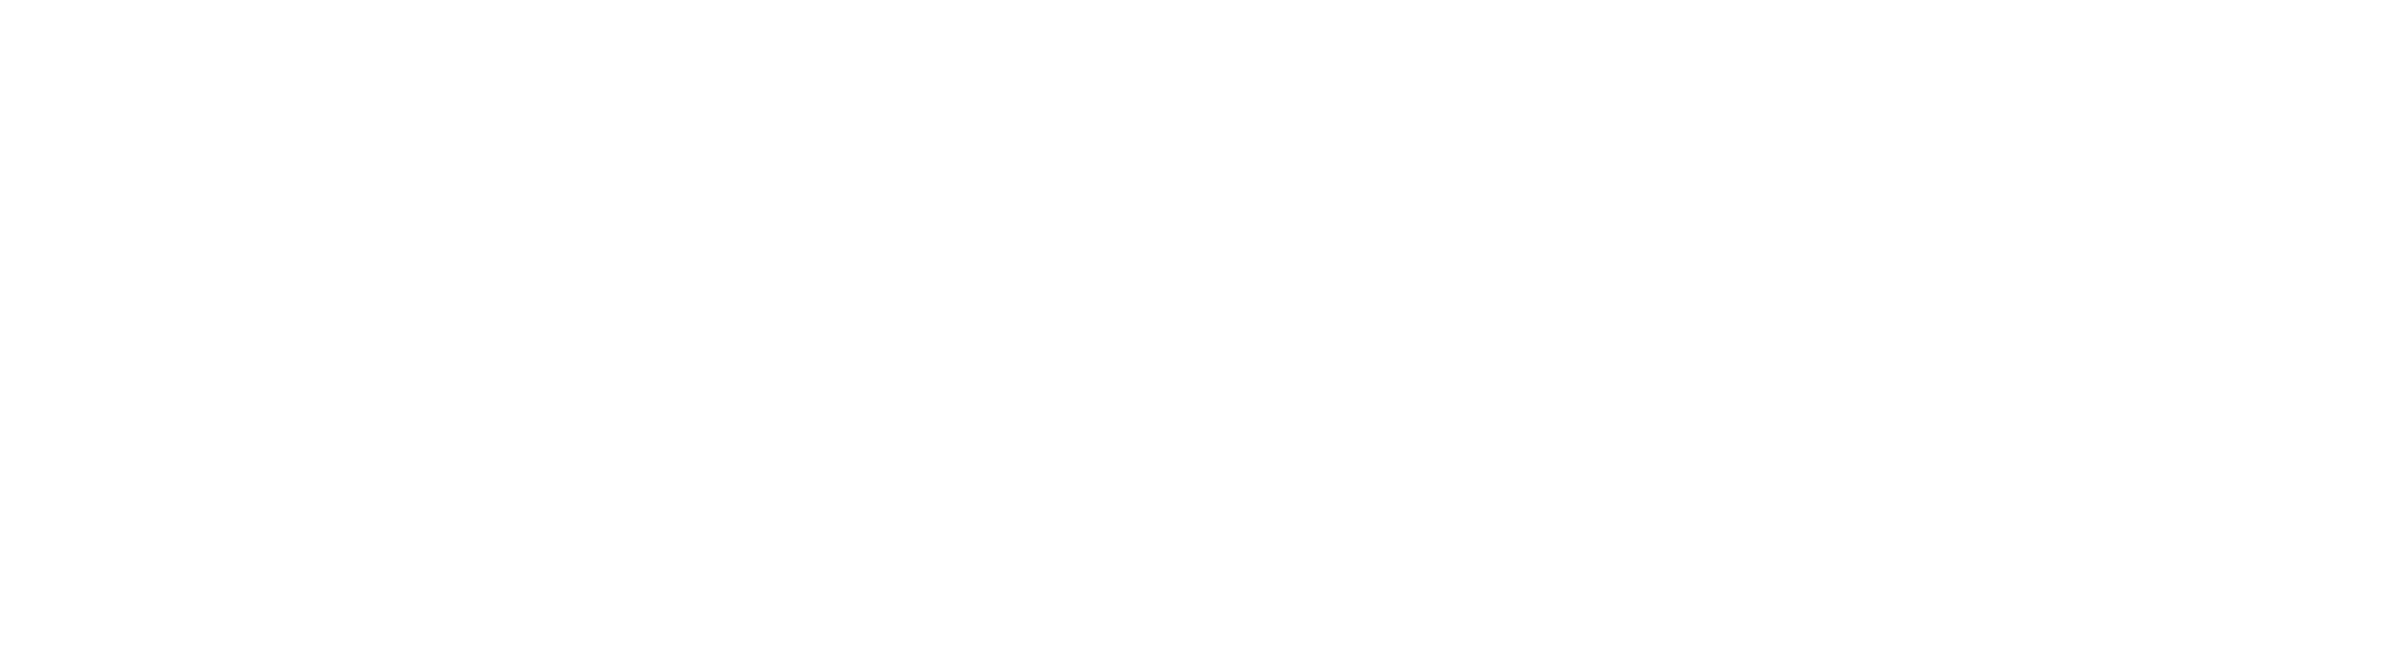
\includegraphics[width=4.6cm]{figuras/usal.png}\par
\vspace{0.75cm}
{\color{sky}\rule{\textwidth}{0.5pt}}\par
\vspace{0.55cm}
{\color{muted}\small\textls[220]{\textsc{Facultad de Ciencias}}\quad·\quad\textls[220]{\textsc{Grado en Física}}}\par
\vspace{1.25cm}
{\color{acc}\textls[260]{\textsc{Ecuaciones Diferenciales}}}\par
\vspace{0.2cm}
{\color{muted}\small\textls[260]{\textsc{Tema 6}}}\par
\vspace{1.25cm}
{\fontsize{27}{33}\selectfont\bfseries Sistemas de EDO lineales\par}
\vspace{0.12cm}
{\fontsize{19}{24}\selectfont\bfseries exponencial de una matriz y forma de Jordan\par}
\vspace{0.55cm}
{\color{acc}\rule{2.4cm}{0.8pt}}\par
\vspace{0.45cm}
{\color{muted}\small\itshape Autovalores y autovectores generalizados\quad·\quad Método canónico\quad·\quad Forma de Jordan\par
Propagador y serie de Dyson\quad·\quad Espacio de fases y estabilidad\par}
\vspace{0.45cm}
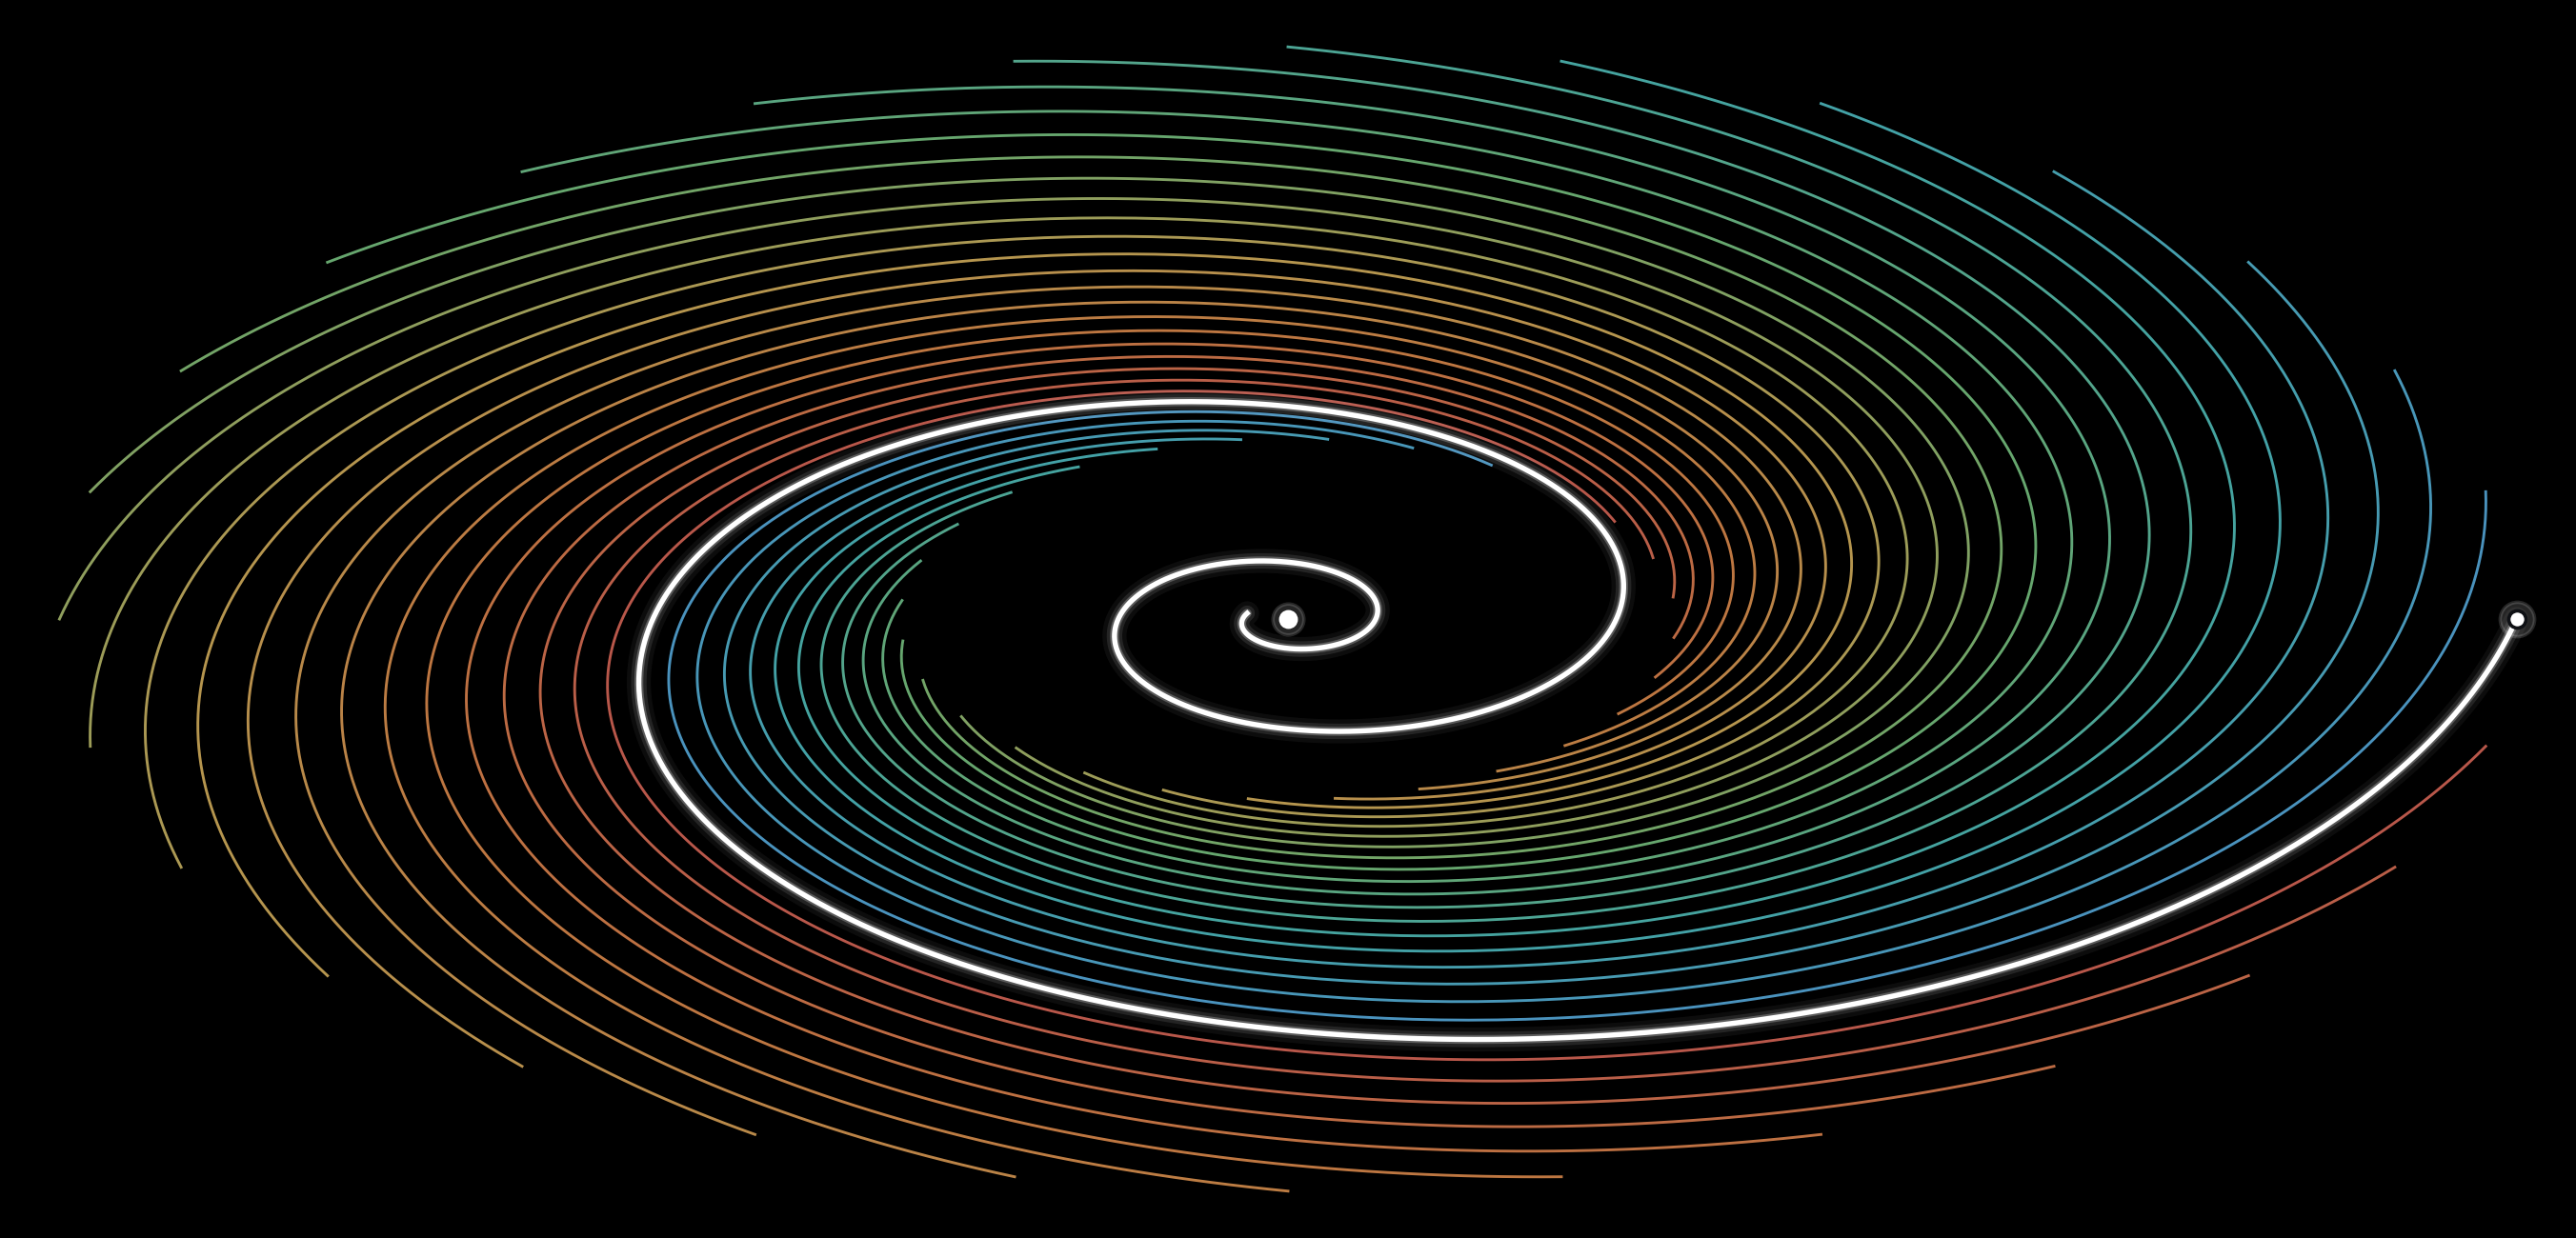
\includegraphics[width=0.86\textwidth]{figuras/portada_t6.png}\par
\vspace{0.35cm}
{\small$\displaystyle \vy\,'=A\,\vy+\vb(t)\quad\Longrightarrow\quad
\vy(t)=\e^{A(t-t_0)}\,\vy_0+\int_{t_0}^{t}\e^{A(t-s)}\,\vb(s)\,\dd s$\par}
\vfill
{\color{sky}\rule{\textwidth}{0.5pt}}\par
\vspace{0.3cm}
\begin{minipage}[t]{0.32\textwidth}\raggedright
{\color{acc}\footnotesize\textls[200]{\textsc{Autor}}}\par\vspace{2pt}
{\small Daniel Martín Guerrero}
\end{minipage}\hfill
\begin{minipage}[t]{0.32\textwidth}\centering
{\color{acc}\footnotesize\textls[200]{\textsc{Profesorado}}}\par\vspace{2pt}
{\small Pilar García Estévez\\ José Beltrán Jiménez\\ María Pérez Garrote}
\end{minipage}\hfill
\begin{minipage}[t]{0.32\textwidth}\raggedleft
{\color{acc}\footnotesize\textls[200]{\textsc{Apuntes formalizados}}}\par\vspace{2pt}
{\small Salamanca, curso 2026/2027}\\[1pt]
{\footnotesize\color{muted}Teoría y seminario de problemas}
\end{minipage}
\end{titlepage}

% =====================================================================
%  ÍNDICE
% =====================================================================
\setcounter{page}{2}
{\hypersetup{linkcolor=fg}\tableofcontents}
\clearpage

% =====================================================================
\section{Sistemas de EDO lineales}\label{sec:sistemas}
% =====================================================================

\begin{motivacion}{Plan del tema}
Un sistema lineal $\vy\,'=A(t)\vy+\vb(t)$ es el análogo vectorial de la EDO lineal del tema~4: la estructura
«homogénea $+$ particular» es la misma y el polinomio característico vuelve a mandar. La novedad está en la
\emph{homogénea con $A$ constante}: su solución es $\e^{At}\vy_0$, y calcular esa exponencial es un problema de
álgebra lineal (autovalores, autovectores generalizados y forma de Jordan, secciones~\ref{sec:autovalores}--\ref{sec:jordan}).
La particular sale por variación de las constantes, que aquí adopta la forma de un propagador
(sección~\ref{sec:completo}). Cerramos con el espacio de fases y la estabilidad (sección~\ref{sec:estabilidad}) y
con la partícula en un campo magnético (sección~\ref{sec:campoB}).
\end{motivacion}

\begin{observacion}[notación]
Los vectores van en negrita, $\vy=(y_1,\dots,y_n)\T$; las matrices, en mayúscula: $A$, $P$, $J$, la identidad
$\Id$. La prima es la derivada respecto de la variable independiente $t$: $\vy\,'=\dd\vy/\dd t$. Cuando citamos un
resultado del tema~4 escribimos «(T4,~4.9)».
\end{observacion}

\subsection{De la mecánica a los sistemas de primer orden}

En mecánica clásica la ecuación de partida es de segundo orden, $\vq\,''=\bm f(\vq,\vq\,',t)$. Introduciendo
$\vp\defeq\vq\,'$ la reescribimos como un sistema de primer orden en el doble de variables:
\begin{equation}\label{eq:hamilton}
\vq\,''=\bm f(\vq,\vq\,',t)
\quad\Longleftrightarrow\quad
\begin{cases}\vq\,'=\vp,\\ \vp\,'=\bm f(\vq,\vp,t),\end{cases}
\qquad
\mat{\vq\\ \vp}'=\mat{\vp\\ \bm f}.
\end{equation}
Es el paso de la mecánica lagrangiana (ecuaciones de segundo orden en $\vq$) a la hamiltoniana (primer orden en
$(\vq,\vp)$). En general, un sistema de EDO es $\vy\,'=\vF(\vy,t)$ con $\vy\in\R^n$.

\begin{proposicion}[Orden $n$ $\Leftrightarrow$ sistema de $n$ ecuaciones]\label{prop:companera}
La EDO lineal $y^{(n)}+a_{n-1}(t)\,y^{(n-1)}+\dots+a_0(t)\,y=b(t)$ equivale al sistema $\vy\,'=A(t)\vy+\vb(t)$ con
$\vy=(y,y',\dots,y^{(n-1)})\T$ y
\begin{equation}\label{eq:companera}
A=\mat{0&1&&\\ &\ddots&\ddots&\\ &&0&1\\ -a_0&-a_1&\cdots&-a_{n-1}},\qquad
\vb=\mat{0\\ \vdots\\ 0\\ b},\qquad
\det(A-\lambda\Id)=(-1)^n\,p(\lambda),
\end{equation}
donde $p(\lambda)=\lambda^n+a_{n-1}\lambda^{n-1}+\dots+a_0$ es el polinomio característico de la EDO.
\end{proposicion}

\begin{demostracion}
\begin{pasos}
\item \emph{Equivalencia.} Las $n-1$ primeras filas dicen $y_k'=y_{k+1}$, es decir, $y_{k+1}=y^{(k)}$; la última es la
EDO despejada.
\item \emph{Polinomio.} Desarrollando $\det(A-\lambda\Id)$ por la última fila (o por inducción en $n$) se obtiene
$(-1)^n(\lambda^n+a_{n-1}\lambda^{n-1}+\dots+a_0)$. Para $n=2$:
$\det\smat{-\lambda&1\\-a_0&-a_1-\lambda}=\lambda^2+a_1\lambda+a_0$.
\end{pasos}
\end{demostracion}

\begin{consejo}{Conexión con el tema 4}
Todo lo del tema 4 es un caso particular de este tema: los autovalores de la matriz compañera \eqref{eq:companera}
son las raíces de $p(\lambda)$, la matriz wronskiana $W$ es la matriz fundamental del sistema y la fórmula de
variación de las constantes (T4,~4.9) es la fórmula \eqref{eq:duhamel} de la sección~\ref{sec:completo}. Si un
ejercicio de sistemas se complica, a veces conviene ir al revés y \emph{eliminar} variables hasta una EDO de orden
$n$ (sección~\ref{sec:eliminacion}).
\end{consejo}

\subsection{Por qué aparecen sistemas lineales: linealización}\label{sec:linealizacion}

Los sistemas lineales aparecen siempre que estudiamos una pequeña perturbación. Sea $\vy\,'=\vF(\vy,t;\alpha)$ con un
parámetro $\alpha\ll1$, y supongamos conocida la solución $\vy_0$ del problema con $\alpha=0$. Buscamos
\begin{equation}
\vy=\vy_0+\alpha\,\vy_1+O(\alpha^2).
\end{equation}

\begin{pasos}
\item \emph{Taylor en $\alpha$ alrededor de $(\vy_0,0)$:}
\begin{equation*}
\vF(\vy_0+\alpha\vy_1,t;\alpha)=\vF(\vy_0,t;0)+\alpha\Big[\Big(\pd{\vF}{\vy}\Big)_{\!0}\vy_1+\Big(\pd{\vF}{\alpha}\Big)_{\!0}\Big]+O(\alpha^2),
\end{equation*}
donde $(\partial\vF/\partial\vy)_0$ es la matriz jacobiana evaluada en $(\vy_0,t;0)$.
\item \emph{Igualando potencias de $\alpha$} en $\vy_0'+\alpha\vy_1'=\vF$:
\begin{equation}\label{eq:linealizada}
\alpha^0:\ \ \vy_0'=\vF(\vy_0,t;0),\qquad
\alpha^1:\ \ \res{\vy_1'=\underbrace{\Big(\pd{\vF}{\vy}\Big)_{\!0}}_{A(t)}\vy_1+\underbrace{\Big(\pd{\vF}{\alpha}\Big)_{\!0}}_{\vb(t)}}
\end{equation}
\end{pasos}
La corrección $\vy_1$ obedece siempre un sistema \emph{lineal}, aunque $\vF$ no lo sea.

\begin{ejemplo}[$\vy\,'=\vy/(1+\alpha\abs{\vy}^2)$]\label{ej:perturbativo}
Para $\alpha\ll1$, $\vF=\vy\,(1-\alpha\abs{\vy}^2)+O(\alpha^2)$, luego
\begin{equation*}
\Big(\pd{\vF}{\vy}\Big)_{\!0}=\Id,\qquad \Big(\pd{\vF}{\alpha}\Big)_{\!0}=-\abs{\vy_0}^2\vy_0
\quad\Longrightarrow\quad
\vy_0'=\vy_0,\qquad \vy_1'=\vy_1-\abs{\vy_0}^2\,\vy_0 .
\end{equation*}
Con $\vy(0)=\vc$: $\vy_0=\e^{t}\vc$ y, por tanto, $\vy_1'-\vy_1=-\abs{\vc}^2\e^{3t}\vc$ con $\vy_1(0)=\bm 0$.
Multiplicando por $\e^{-t}$: $(\e^{-t}\vy_1)'=-\abs{\vc}^2\e^{2t}\vc$, e integrando,
\begin{equation}\label{eq:pert-sol}
\vy\simeq\e^{t}\vc-\frac{\alpha}{2}\abs{\vc}^2\big(\e^{3t}-\e^{t}\big)\vc .
\end{equation}
\end{ejemplo}

\begin{observacion}[errata del manuscrito]
En los apuntes de clase aparece $\vy_1'=\vy_1-\vy_0^{\,2}\,\vy_1$. El término fuente es
$(\partial\vF/\partial\alpha)_0=-\abs{\vy_0}^2\vy_0$ (no depende de $\vy_1$): la ecuación de orden $\alpha$ es lineal
\emph{e inhomogénea}, con $A=\Id$ y $\vb=-\abs{\vy_0}^2\vy_0$, como exige \eqref{eq:linealizada}.
\end{observacion}

\begin{figure}[!htbp]
\centering
\begin{tikzpicture}
\begin{axis}[oscuro,width=9.2cm,height=5.6cm,xmin=0,xmax=1.27,ymin=0.8,ymax=3.6,
  axis lines=left,xtick={0,0.4,0.8,1.2},ytick={1,2,3},xlabel={$t$},ylabel={$y$},clip=false,
  every axis x label/.style={at={(ticklabel* cs:1.02)},anchor=west},
  every axis y label/.style={at={(ticklabel* cs:1.02)},anchor=south}]
\addplot[muted,dashed,line width=0.7pt,domain=0:1.2]{exp(x)};
\addplot[gold,domain=1:2.8,variable=\y] ({ln(\y)+0.025*(\y*\y-1)},{\y});
\addplot[acc,domain=0:1.2]{exp(x)+0.025*(exp(x)-exp(3*x))};
\node[anchor=west,font=\scriptsize,muted] at (axis cs:1.21,3.32) {$y_0=\e^{t}$};
\node[anchor=west,font=\scriptsize,gold] at (axis cs:1.21,2.86) {exacta};
\node[anchor=west,font=\scriptsize,acc] at (axis cs:1.21,2.42) {$y_0+\alpha y_1$};
\end{axis}
\end{tikzpicture}
\caption{Ejemplo~\ref{ej:perturbativo} en una dimensión con $c=1$, $\alpha=0.05$. Dorado: solución exacta
$\ln y+\frac{\alpha}{2}(y^2-1)=t$; azul: aproximación \eqref{eq:pert-sol}; gris: orden cero. El error de $y_0+\alpha y_1$
es $O(\alpha^2\e^{5t})$ y crece con $t$.}
\label{fig:perturbativo}
\end{figure}

\subsection{Estructura de la solución}

\begin{definicion}[Sistema lineal]\label{def:sistema}
Sea $I\subseteq\R$ un intervalo, $A\colon I\to\R^{n\times n}$ y $\vb\colon I\to\R^n$ continuas. El sistema
\begin{equation}\label{eq:sistema}
\vy\,'=A(t)\,\vy+\vb(t),\qquad
\left\{\begin{aligned}
y_1'&=a_{11}(t)\,y_1+\dots+a_{1n}(t)\,y_n+b_1(t),\\[-2pt]
&\ \,\vdots\\[-2pt]
y_n'&=a_{n1}(t)\,y_1+\dots+a_{nn}(t)\,y_n+b_n(t),
\end{aligned}\right.
\end{equation}
es un \emph{sistema lineal de primer orden}. Es \emph{homogéneo} si $\vb\equiv\bm 0$; $\vb$ es la \emph{fuente}.
\end{definicion}

\begin{teorema}[Estructura de la solución]\label{teo:estructura}
Sea $L[\vy]\defeq\vy\,'-A\vy$.
\begin{enumerate}
\item Para cada $(t_0,\vy_0)\in I\times\R^n$ existe una única solución de \eqref{eq:sistema} con $\vy(t_0)=\vy_0$ (se admite).
\item $\ker L$ es un espacio vectorial de dimensión $n$. Si $\vy_1,\dots,\vy_n$ es una base, la \emph{matriz
fundamental} $\Phi=(\vy_1\,|\cdots|\,\vy_n)$ cumple $\Phi'=A\Phi$ y $\det\Phi(t)\neq0$ para todo $t$.
\item Si $\vy_p$ es una solución de \eqref{eq:sistema}, todas las soluciones son
\begin{equation}\label{eq:yh+yp}
\vy=\vy_h+\vy_p=\Phi(t)\,\vk+\vy_p,\qquad \vk\in\R^n.
\end{equation}
\end{enumerate}
\end{teorema}

\begin{demostracion}
\begin{pasos}
\item \emph{Linealidad.} $L[\alpha\vy+\beta\vz]=\alpha L[\vy]+\beta L[\vz]$, luego $\ker L$ es subespacio.
\item \emph{Dimensión.} La aplicación $\vy\mapsto\vy(t_0)$, $\ker L\to\R^n$, es lineal, sobreyectiva (existencia) e
inyectiva (unicidad): es un isomorfismo. Es el mismo argumento que (T4, teorema~1.4).
\item \emph{$\det\Phi\neq0$.} Si $\Phi(t_1)\vk=\bm 0$ con $\vk\neq\bm0$, la solución $\Phi\vk$ y la nula coinciden en
$t_1$; por unicidad $\Phi\vk\equiv\bm0$, contra la independencia.
\item \emph{Estructura.} $L[\vy-\vy_p]=\vb-\vb=\bm0\Rightarrow\vy-\vy_p\in\ker L$.
\end{pasos}
\end{demostracion}

\begin{recordatorio}[Abel--Liouville en versión matricial]
El wronskiano $w=\det\Phi$ cumple $w'=\tr A\;w$, luego $w(t)=w(t_0)\exp\!\int_{t_0}^{t}\tr A(s)\,\dd s$. Para la
matriz compañera, $\tr A=-a_{n-1}$ y se recupera (T4, teorema~1.13). Con $A$ constante,
$\det\e^{At}=\e^{t\tr A}$, identidad que usaremos para comprobar cálculos.
\end{recordatorio}

\subsection{Método de eliminación}\label{sec:eliminacion}

Para $n=2$ o $3$ podemos reducir el sistema a una única EDO de orden $n$: derivamos una ecuación y sustituimos
las demás. Con $n=2$ y coeficientes variables,
\begin{equation*}
y_1'=a_{11}y_1+a_{12}y_2,\qquad y_2'=a_{21}y_1+a_{22}y_2\qquad(a_{12}\neq0).
\end{equation*}

\begin{pasos}
\item \emph{Derivamos la primera} y sustituimos $y_2'$ con la segunda:
$y_1''=a_{11}'y_1+a_{11}y_1'+a_{12}'y_2+a_{12}\,(a_{21}y_1+a_{22}y_2)$.
\item \emph{Despejamos} $y_2$ de la primera: $y_2=\big(y_1'-a_{11}y_1\big)/a_{12}$.
\item \emph{Sustituyendo},
\begin{equation}\label{eq:eliminacion}
y_1''=\Big(a_{11}+a_{22}+\frac{a_{12}'}{a_{12}}\Big)y_1'
+\Big(a_{11}'+a_{12}a_{21}-a_{11}a_{22}-\frac{a_{11}a_{12}'}{a_{12}}\Big)y_1 .
\end{equation}
\end{pasos}
Con coeficientes constantes queda $y_1''-(\tr A)\,y_1'+(\det A)\,y_1=0$, cuyo polinomio es $\det(A-\lambda\Id)$:
eliminar y diagonalizar son el mismo cálculo. Lo usamos en el problema~\ref{prob:2}.

% =====================================================================
\section{Coeficientes constantes: el método de autovalores}\label{sec:autovalores}
% =====================================================================

Desde aquí $A\in\R^{n\times n}$ es constante y estudiamos la homogénea $\vy\,'=A\vy$. Interesa en sí misma
(modos normales, estabilidad) y porque, como en el tema 4, es el primer paso para la completa.

\subsection{El ansatz exponencial}

\begin{proposicion}[Soluciones exponenciales]\label{prop:ansatz}
$\vy(t)=\e^{\lambda t}\vv$, con $\vv\neq\bm0$ constante, es solución de $\vy\,'=A\vy$ si y sólo si $A\vv=\lambda\vv$.
\end{proposicion}

\begin{demostracion}
$\vy\,'=\lambda\e^{\lambda t}\vv$ y $A\vy=\e^{\lambda t}A\vv$. Como $\e^{\lambda t}\neq0$, ambas coinciden si y sólo si
$A\vv=\lambda\vv$.
\end{demostracion}

Los $\lambda$ son las raíces del \emph{polinomio característico} $p_A(\lambda)\defeq\det(A-\lambda\Id)$.

\subsection{Autovalores simples}

\begin{teorema}[Base de autovectores]\label{teo:simples}
Si $A$ tiene $n$ autovectores independientes $\vv_1,\dots,\vv_n$ (en particular, si sus $n$ autovalores son
distintos), la solución general de $\vy\,'=A\vy$ es
\begin{equation}\label{eq:simples}
\vy(t)=\sum_{j=1}^{n}k_j\,\e^{\lambda_jt}\,\vv_j,\qquad k_j\in\C .
\end{equation}
\end{teorema}

\begin{demostracion}
Cada sumando es solución (proposición~\ref{prop:ansatz}). En $t=0$ la matriz $\Phi(0)=(\vv_1|\cdots|\vv_n)$ es
invertible, luego las $n$ soluciones son independientes (teorema~\ref{teo:estructura}). Autovectores de autovalores
distintos son independientes (resultado de álgebra lineal que se admite).
\end{demostracion}

\begin{ejemplo}[$y_1'=-y_1-2y_2,\ y_2'=3y_1+4y_2$]\label{ej:2-1}
\begin{pasos}
\item \emph{Polinomio:} $\det\smat{-1-\lambda&-2\\3&4-\lambda}=\lambda^2-3\lambda+2=(\lambda-1)(\lambda-2)$.
\item \emph{Autovectores:} $(A-\Id)\vv=\bm0$: $\smat{-2&-2\\3&3}\vv=\bm0\Rightarrow\vv_1=(1,-1)\T$;
$\ (A-2\Id)\vv=\bm0$: $\smat{-3&-2\\3&2}\vv=\bm0\Rightarrow\vv_2=(2,-3)\T$.
\item \emph{Solución:}
\begin{equation*}
\vy=k_1\e^{t}\mat{1\\-1}+k_2\e^{2t}\mat{2\\-3}=\mat{k_1\e^{t}+2k_2\e^{2t}\\ -k_1\e^{t}-3k_2\e^{2t}}.
\end{equation*}
\end{pasos}
\end{ejemplo}

\begin{observacion}[errata de los apuntes digitales]
En el ejemplo 2.1 de los apuntes de teoría aparece $a_{11}=+1$. Con ese signo $p_A(\lambda)=\lambda^2-5\lambda+10$,
sin raíces reales, y $(1,-1)\T$ no es autovector. El polinomio $(\lambda-1)(\lambda-2)$ y los autovectores dados
corresponden a $a_{11}=-1$, que es además el problema~2 del seminario.
\end{observacion}

\subsection{Autovalores complejos}

Si $A$ es real y $\lambda=\alpha+\iu\beta$ ($\beta\neq0$) es autovalor con $\vv=\vp+\iu\vq$, conjugando
$A\vv=\lambda\vv$ obtenemos $A\vv^*=\lambda^*\vv^*$: los autovalores y autovectores complejos van por parejas.

\begin{proposicion}[Soluciones reales]\label{prop:complejas}
Las partes real e imaginaria de $\e^{\lambda t}\vv$ son soluciones reales independientes:
\begin{equation}\label{eq:complejas}
\vy=c_1\,\e^{\alpha t}\big[\vp\cos\beta t-\vq\sen\beta t\big]+c_2\,\e^{\alpha t}\big[\vp\sen\beta t+\vq\cos\beta t\big],
\qquad c_1,c_2\in\R .
\end{equation}
\end{proposicion}

\begin{demostracion}
\begin{pasos}
\item \emph{Desarrollo:} $\e^{\lambda t}\vv=\e^{\alpha t}(\cos\beta t+\iu\sen\beta t)(\vp+\iu\vq)
=\e^{\alpha t}\big[\vp\cos\beta t-\vq\sen\beta t\big]+\iu\,\e^{\alpha t}\big[\vp\sen\beta t+\vq\cos\beta t\big]$.
\item \emph{Son soluciones:} como $A$ es real, $\Re$ e $\Im$ conmutan con $\dd/\dd t-A$.
\item \emph{Independencia:} generan el mismo espacio que $\e^{\lambda t}\vv$ y $\e^{\lambda^*t}\vv^*$, que son
independientes por el teorema~\ref{teo:simples}.
\end{pasos}
\end{demostracion}

\subsection{Autovalores múltiples: autovectores generalizados}\label{sec:multiples}

Si $\lambda$ tiene multiplicidad algebraica $h>1$ y no hay $h$ autovectores independientes, el ansatz
$\e^{\lambda t}\vv$ se queda corto. Como en el tema~4 (raíces múltiples $\Rightarrow$ factor $x^k$), probamos
polinomios en $t$.

\begin{pasos}
\item \emph{Primera solución:} $\vy_1=\e^{\lambda t}\vv_1$ con $(A-\lambda\Id)\vv_1=\bm0$.
\item \emph{Ansatz lineal:} $\vy_2=(\vv_2+t\,\vv_1)\,\e^{\lambda t}$. Derivando y aplicando $A$:
\begin{equation*}
\vy_2'=\big[\lambda(\vv_2+t\vv_1)+\vv_1\big]\e^{\lambda t},\qquad
A\vy_2=\big[A\vv_2+t\,\lambda\vv_1\big]\e^{\lambda t}.
\end{equation*}
Igualando: $A\vv_2=\lambda\vv_2+\vv_1$, es decir,
\begin{equation}\label{eq:cadena2}
(A-\lambda\Id)\,\vv_2=\vv_1\qquad(\text{autovector generalizado}).
\end{equation}
\item \emph{Ansatz cuadrático:} $\vy_3=\big(\vv_3+t\,\vv_2+\tfrac12t^2\vv_1\big)\e^{\lambda t}$. Ahora
$\vy_3'=\big[\lambda\big(\vv_3+t\vv_2+\tfrac12t^2\vv_1\big)+\vv_2+t\vv_1\big]\e^{\lambda t}$, y al igualar con
$A\vy_3$ los términos en $t^2$ y $t$ se cancelan por \eqref{eq:cadena2}; el de orden cero da $(A-\lambda\Id)\vv_3=\vv_2$.
\end{pasos}

El patrón es una \emph{cadena de Jordan}. Con $N\defeq A-\lambda\Id$:
\begin{equation}\label{eq:cadena}
\vv_h\ \xrightarrow{\ N\ }\ \vv_{h-1}\ \xrightarrow{\ N\ }\ \cdots\ \xrightarrow{\ N\ }\ \vv_1\ \xrightarrow{\ N\ }\ \bm0,
\qquad \vv_j=N^{h-j}\vv_h .
\end{equation}

\begin{teorema}[Soluciones de una cadena]\label{teo:cadena}
Si $N^h\vv_h=\bm0$, entonces
\begin{equation}\label{eq:sol-cadena}
\res{\vy(t)=\e^{\lambda t}\sum_{k=0}^{h-1}\frac{t^k}{k!}\,N^k\vv_h
=\e^{\lambda t}\Big(\vv_h+t\,\vv_{h-1}+\frac{t^2}{2!}\vv_{h-2}+\dots+\frac{t^{h-1}}{(h-1)!}\vv_1\Big)}
\end{equation}
es solución de $\vy\,'=A\vy$, con $\vy(0)=\vv_h$. Si $\vv_h$ recorre $\ker N^h$, se obtiene todo el subespacio de
soluciones asociado a $\lambda$.
\end{teorema}

\begin{demostracion}
\begin{pasos}
\item \emph{Derivando} \eqref{eq:sol-cadena}:
$\vy\,'=\lambda\vy+\e^{\lambda t}\sum_{k=1}^{h-1}\frac{t^{k-1}}{(k-1)!}N^k\vv_h$.
\item \emph{Aplicando $N$:} $N\vy=\e^{\lambda t}\sum_{k=0}^{h-1}\frac{t^k}{k!}N^{k+1}\vv_h
=\e^{\lambda t}\sum_{k=1}^{h-1}\frac{t^{k-1}}{(k-1)!}N^{k}\vv_h$, pues el término $k=h-1$ da $N^h\vv_h=\bm0$.
\item \emph{Luego} $\vy\,'=\lambda\vy+N\vy=A\vy$. La última afirmación se sigue de que
$\dim\ker N^h=h$ (sección~\ref{sec:jordan}).
\end{pasos}
\end{demostracion}

\begin{observacion}[relación con los apuntes digitales]
En los apuntes de teoría la solución se escribe $\vy=\e^{\lambda t}\sum_{j=1}^{h}a_j\,t^{h-j}\,\bm Y_j$ con
$\bm Y_j=(A-\lambda\Id)\bm Y_{j+1}$, y la recurrencia $(A-\lambda\Id)\,a_{j+1}\bm Y_{j+1}=(h-j)\,a_j\bm Y_j$ da
$a_j=a_h/(h-j)!$. Es \eqref{eq:sol-cadena} con $a_h=1$. La cadena se calcula \emph{descendiendo} desde $\vv_h$
porque $A-\lambda\Id$ no es invertible: no se puede «subir» despejando.
\end{observacion}

\begin{ejemplo}[raíz triple, $N$ de índice 3]\label{ej:2-2}
$A=\smat{2&1&1\\1&2&0\\-1&0&2}$.
\begin{pasos}
\item \emph{Polinomio:} $p_A(\lambda)=-(\lambda-2)^3$, raíz triple $\lambda=2$.
\item \emph{Potencias de $N=A-2\Id$:}
\begin{equation*}
N=\mat{0&1&1\\1&0&0\\-1&0&0},\qquad
N^2=\mat{0&0&0\\0&1&1\\0&-1&-1},\qquad N^3=0 .
\end{equation*}
\item \emph{Cadena:} como $N^3=0$, $\vv_3=\vc=(c_1,c_2,c_3)\T$ es arbitrario y
$\vv_2=N\vc=(c_2+c_3,\ c_1,\ -c_1)\T$, $\vv_1=N^2\vc=(0,\ c_2+c_3,\ -c_2-c_3)\T$.
\item \emph{Solución} por \eqref{eq:sol-cadena}:
\begin{equation*}
\vy=\e^{2t}\Big(\vv_3+t\,\vv_2+\tfrac{t^2}{2}\vv_1\Big)
=\e^{2t}\mat{c_1+t\,(c_2+c_3)\\[1pt] c_2+t\,c_1+\tfrac{t^2}{2}(c_2+c_3)\\[1pt] c_3-t\,c_1-\tfrac{t^2}{2}(c_2+c_3)}.
\end{equation*}
\end{pasos}
Los apuntes digitales dan el doble de este vector ($a_1=1$, $a_2=a_3=2$): es la misma familia.
\end{ejemplo}

\begin{ejemplo}[raíz triple, $N$ de índice 2]\label{ej:2-3}
$A=\smat{6&-6&5\\14&-13&10\\7&-6&4}$.
\begin{pasos}
\item \emph{Polinomio:} $p_A(\lambda)=-(\lambda+1)^3$.
\item \emph{Nilpotencia:} $N=A+\Id=\smat{7&-6&5\\14&-12&10\\7&-6&5}$ tiene rango 1, con todas las columnas
proporcionales a $(1,2,1)\T$, y $N^2=0$ porque $(7,-6,5)\cdot(1,2,1)=0$.
\item \emph{Solución:} con $\vc$ arbitrario, $N\vc=(7c_1-6c_2+5c_3)\,(1,2,1)\T$ y
\begin{equation*}
\vy=\e^{-t}\big(\vc+t\,N\vc\big)=\e^{-t}\mat{c_1+t\,(7c_1-6c_2+5c_3)\\ c_2+2t\,(7c_1-6c_2+5c_3)\\ c_3+t\,(7c_1-6c_2+5c_3)}.
\end{equation*}
\end{pasos}
\end{ejemplo}

% =====================================================================
\section{Método canónico: la exponencial de una matriz}\label{sec:canonico}
% =====================================================================

\subsection{Definición y propiedades}

Para la ecuación escalar $f'=af$ la solución es $f=\e^{at}f_0$. El método canónico copia esta fórmula.

\begin{definicion}[Exponencial de una matriz]\label{def:exp}
Para $A\in\C^{n\times n}$,
\begin{equation}\label{eq:exp}
\e^{At}\defeq\sum_{n=0}^{\infty}\frac{t^n}{n!}A^n=\Id+tA+\frac{t^2}{2!}A^2+\frac{t^3}{3!}A^3+\cdots
\end{equation}
La serie converge absolutamente para todo $t$, pues $\norm{A^n}\le\norm{A}^n$ (se admite).
\end{definicion}

\begin{teorema}[Solución de la homogénea]\label{teo:canonico}
$\dfrac{\dd}{\dd t}\e^{At}=A\,\e^{At}=\e^{At}A$, y la solución de $\vy\,'=A\vy$, $\vy(t_0)=\vy_0$, es
\begin{equation}\label{eq:canonico}
\res{\vy(t)=\e^{A(t-t_0)}\,\vy_0}
\end{equation}
\end{teorema}

\begin{demostracion}
\begin{pasos}
\item \emph{Derivando término a término} (convergencia uniforme en compactos):
\begin{equation*}
\frac{\dd}{\dd t}\e^{At}=\sum_{n=1}^{\infty}\frac{n\,t^{n-1}}{n!}A^n=\sum_{n=1}^{\infty}\frac{t^{n-1}}{(n-1)!}A^n
\overset{k=n-1}{=}\sum_{k=0}^{\infty}\frac{t^k}{k!}A^{k+1}=A\sum_{k=0}^{\infty}\frac{t^k}{k!}A^k=A\,\e^{At}.
\end{equation*}
\item \emph{Condición inicial:} $\e^{A\cdot0}=\Id$. Por unicidad, \eqref{eq:canonico} es la solución.
\end{pasos}
\end{demostracion}

Así, $\e^{At}$ es la matriz fundamental con $\Phi(0)=\Id$: sus columnas son las soluciones que parten de
$\bm e_1,\dots,\bm e_n$. Todo el problema se reduce a \emph{calcular} $\e^{At}$.

\begin{proposicion}[Propiedades]\label{prop:propiedades-exp}
\begin{enumerate}
\item Si $[X,Y]\defeq XY-YX=0$, entonces $\e^{X+Y}=\e^{X}\e^{Y}$. En particular $\e^{A(t+s)}=\e^{At}\e^{As}$ y
$(\e^{At})^{-1}=\e^{-At}$.
\item $\e^{P^{-1}AP\,t}=P^{-1}\e^{At}P$ para cualquier $P$ invertible.
\item $\e^{\diag(\lambda_1,\dots,\lambda_n)t}=\diag(\e^{\lambda_1t},\dots,\e^{\lambda_nt})$.
\item Si $N^p=0$, $\e^{Nt}=\sum_{k=0}^{p-1}\frac{t^k}{k!}N^k$ (la serie es finita).
\end{enumerate}
\end{proposicion}

\begin{demostracion}
(1) Si $X$ e $Y$ conmutan vale el binomio de Newton, $(X+Y)^n=\sum_k\binom nk X^kY^{n-k}$, y el producto de Cauchy
de las dos series da $\e^{X}\e^{Y}$. (2) $(P^{-1}AP)^n=P^{-1}A^nP$ término a término. (3) $D^n=\diag(\lambda_j^n)$.
(4) Los términos con $k\ge p$ se anulan.
\end{demostracion}

\begin{observacion}[fórmula de Baker--Campbell--Hausdorff]
Si $[X,Y]\neq0$, $\e^{X}\e^{Y}=\e^{Z}$ con
\begin{equation*}
Z=X+Y+\tfrac12[X,Y]+\tfrac1{12}\big([X,[X,Y]]+[Y,[Y,X]]\big)+\cdots
\end{equation*}
y en general $\e^{X+Y}\neq\e^{X}\e^{Y}$. Por eso necesitaremos descomponer $A$ en dos partes que \emph{conmuten}.
\end{observacion}

\subsection{Reducción a la forma de Jordan}

Si $A$ fuese diagonal, la propiedad~3 daría $\e^{At}$ inmediatamente. En general la diagonalizamos «lo más
posible» con un cambio de base.

\begin{pasos}
\item \emph{Cambio de base:} $\vy=P\vz$, con $P$ invertible cuyas columnas son autovectores (generalizados) de $A$.
\item \emph{Sistema en la nueva base:} $(P\vz)'=AP\vz\ \Rightarrow\ \vz\,'=P^{-1}AP\,\vz\eqqcolon J\vz$.
\item \emph{Solución:} $\vz=\e^{J(t-t_0)}\vz_0$ y, volviendo,
\begin{equation}\label{eq:PJP}
\res{\vy(t)=P\,\e^{J(t-t_0)}P^{-1}\,\vy_0=P\,\e^{J(t-t_0)}\vk},\qquad \vk\defeq P^{-1}\vy_0 .
\end{equation}
\end{pasos}

El teorema de Jordan (sección~\ref{sec:jordan}) asegura que siempre podemos elegir $P$ de forma que
\begin{equation}\label{eq:DN}
J=D+N,\qquad D=\diag(\lambda_1,\dots,\lambda_n),\qquad N^p=0,\qquad [D,N]=0 .
\end{equation}
Como $D$ y $N$ conmutan, la propiedad~1 permite separar:
\begin{equation}\label{eq:eJt}
\begin{aligned}
\e^{J(t-t_0)}=\e^{D(t-t_0)}\e^{N(t-t_0)}
&=\mat{\e^{\lambda_1(t-t_0)}&&\\&\ddots&\\&&\e^{\lambda_n(t-t_0)}}\\
&\quad\times\Big[\Id+N(t-t_0)+\tfrac12N^2(t-t_0)^2+\dots+\tfrac{1}{(p-1)!}N^{p-1}(t-t_0)^{p-1}\Big].
\end{aligned}
\end{equation}

\begin{observacion}[por qué $D$ y $N$ conmutan]
$N$ sólo tiene unos en la superdiagonal \emph{dentro} de cada bloque, y en cada bloque $D$ es múltiplo de la
identidad, $\lambda_i\Id$, que conmuta con todo. Si mezclásemos autovalores distintos en un mismo bloque, $[D,N]\neq0$.
\end{observacion}

\subsection{Dos ejemplos de los apuntes}

\begin{ejemplo}[raíces simples, $A=\smat{-3&-3\\1&1}$]\label{ej:3-1}
\begin{pasos}
\item \emph{Polinomio:} $\det\smat{-3-\lambda&-3\\1&1-\lambda}=\lambda^2+2\lambda=\lambda(\lambda+2)$.
\item \emph{Autovectores:} $A\vv_1=\bm0\Rightarrow\vv_1=(1,-1)\T$; $\ (A+2\Id)\vv_2=\bm0$:
$\smat{-1&-3\\1&3}\vv_2=\bm0\Rightarrow\vv_2=(3,-1)\T$.
\item \emph{Cambio de base:} $P=\smat{1&3\\-1&-1}$, $\det P=2$, $P^{-1}=\frac12\smat{-1&-3\\1&1}$ y
$J=P^{-1}AP=\diag(0,-2)$.
\item \emph{Solución:}
\begin{equation*}
\vy=P\e^{Jt}\vk=\mat{1&3\\-1&-1}\mat{1&0\\0&\e^{-2t}}\mat{k_1\\k_2}=\mat{k_1+3k_2\e^{-2t}\\-k_1-k_2\e^{-2t}}.
\end{equation*}
\end{pasos}
El autovalor nulo produce una \emph{recta de equilibrios}, $\vy=k_1(1,-1)\T$ (figura~\ref{fig:fases}f).
\end{ejemplo}

\begin{ejemplo}[raíz doble no diagonalizable, $A=\smat{-3&-4\\1&1}$]\label{ej:4-1}
\begin{pasos}
\item \emph{Polinomio:} $\det\smat{-3-\lambda&-4\\1&1-\lambda}=\lambda^2+2\lambda+1=(\lambda+1)^2$.
\item \emph{Nilpotencia:} $N=A+\Id=\smat{-2&-4\\1&2}\neq0$, $\rg N=1$, y $N^2=0$ (Cayley--Hamilton).
\item \emph{Cadena:} $\vv_2=(1,0)\T$ (cualquiera con $N\vv_2\neq\bm0$) y $\vv_1=N\vv_2=(-2,1)\T$.
\item \emph{Cambio de base:} $P=(\vv_1|\vv_2)=\smat{-2&1\\1&0}$, $P^{-1}=\smat{0&1\\1&2}$ y
\begin{equation*}
J=P^{-1}AP=\mat{-1&1\\0&-1},\qquad
\e^{Jt}=\e^{-t}\mat{1&t\\0&1}.
\end{equation*}
\item \emph{Solución:}
\begin{equation*}
\vy=P\e^{Jt}\vk=\e^{-t}\mat{-2&1\\1&0}\mat{k_1+t\,k_2\\k_2}=\e^{-t}\mat{-2k_1+(1-2t)\,k_2\\ k_1+t\,k_2}.
\end{equation*}
\end{pasos}
Es el problema~\ref{prob:1} del seminario, donde además calculamos $\e^{At}$ explícitamente.
\end{ejemplo}

% =====================================================================
\section{Forma canónica de Jordan}\label{sec:jordan}
% =====================================================================

\subsection{Multiplicidades y el teorema de Jordan}

\begin{definicion}[Multiplicidades]\label{def:multiplicidades}
Sea $p_A(\lambda)=\prod_i(\lambda_i-\lambda)^{h_i}$ con $\lambda_i$ distintos. Llamamos
\begin{itemize}
\item \emph{multiplicidad algebraica} de $\lambda_i$ a $h_i$;
\item \emph{multiplicidad geométrica} de $\lambda_i$ a $g_i\defeq\dim\ker(A-\lambda_i\Id)$, el número de autovectores
independientes. Siempre $1\le g_i\le h_i$;
\item \emph{subespacio propio generalizado} a $E_i\defeq\ker(A-\lambda_i\Id)^{h_i}$, con $\dim E_i=h_i$.
\end{itemize}
\end{definicion}

\begin{teorema}[Forma canónica de Jordan]\label{teo:jordan}
Para toda $A\in\C^{n\times n}$ existe $P$ invertible tal que $P^{-1}AP=J=\diag(J_1,\dots,J_r)$, con bloques
\begin{equation}\label{eq:bloque}
J_k=\mat{\lambda&1&&\\&\lambda&\ddots&\\&&\ddots&1\\&&&\lambda}=\lambda\Id+N_k,\qquad N_k^{\,m_k}=0 .
\end{equation}
Para cada $\lambda_i$ hay exactamente $g_i$ bloques, y la suma de sus tamaños es $h_i$. Las columnas de $P$
correspondientes a un bloque forman una cadena \eqref{eq:cadena}. $A$ es diagonalizable si y sólo si $g_i=h_i$ para
todo $i$. (Se admite.)
\end{teorema}

\begin{recordatorio}[Cayley--Hamilton]
Toda matriz anula su polinomio característico: $p_A(A)=0$. Si $p_A(\lambda)=(\lambda-\lambda_i)^{h}\,\tilde p(\lambda)$,
entonces $(A-\lambda_i\Id)^{h}$ se anula sobre $E_i$; si además $\lambda_i$ es el único autovalor
($p_A=\pm(\lambda-\lambda_i)^n$), $(A-\lambda_i\Id)^n=0$ en todo $\C^n$. Por eso en los ejemplos~\ref{ej:2-2}
y~\ref{ej:2-3} no debe sorprender que $N^3=0$: lo garantiza el teorema.
\end{recordatorio}

\begin{figure}[!htbp]
\centering
\begin{tikzpicture}[x=1cm,y=1cm,
  nodo/.style={circle,draw=acc,fill=boxbg,line width=0.6pt,minimum size=9mm,inner sep=0pt,font=\small},
  nodov/.style={circle,draw=muted,fill=boxbg,line width=0.5pt,minimum size=9mm,inner sep=0pt,font=\small}]
\node[nodo] (v3) at (0,0) {$\vv_3$};
\node[nodo] (v2) at (2.6,0) {$\vv_2$};
\node[nodo] (v1) at (5.2,0) {$\vv_1$};
\node[nodov] (z) at (7.8,0) {$\bm 0$};
\draw[flecha,acc] (v3) -- node[above=2pt,font=\scriptsize,fg]{$N$} (v2);
\draw[flecha,acc] (v2) -- node[above=2pt,font=\scriptsize,fg]{$N$} (v1);
\draw[flecha,muted] (v1) -- node[above=2pt,font=\scriptsize,fg]{$N$} (z);
\node[font=\scriptsize,muted,below=7pt of v3,align=center] {$N^3\vv_3=\bm0$\\[-1pt]$N\vv_3\ne\bm0,\ N^2\vv_3\ne\bm0$};
\node[font=\scriptsize,muted,below=7pt of v1,align=center] {autovector};
\node[font=\small] at (3.9,-2.0) {$\e^{At}\vv_3=\e^{\lambda t}\big(\vv_3+t\,\vv_2+\tfrac{t^2}{2}\vv_1\big),
\qquad A(\vv_1|\vv_2|\vv_3)=(\vv_1|\vv_2|\vv_3)\smat{\lambda&1&0\\0&\lambda&1\\0&0&\lambda}$};
\end{tikzpicture}
\caption{Cadena de Jordan de longitud 3 con $N=A-\lambda\Id$. Se construye de izquierda a derecha, eligiendo
$\vv_3\notin\ker N^2$; cada columna de $P$ es la imagen por $N$ de la siguiente.}
\label{fig:cadena}
\end{figure}

\subsection{Caso bidimensional}

Sean $\lambda_1,\lambda_2$ las raíces de $p_A$.
\begin{itemize}
\item $\lambda_1\neq\lambda_2$: $J=D=\diag(\lambda_1,\lambda_2)$.
\item $\lambda_1=\lambda_2=\lambda$ y $g=2$: $A=\lambda\Id$ ya es diagonal (cualquier vector es autovector).
\item $\lambda_1=\lambda_2=\lambda$ y $g=1$:
$J=\smat{\lambda&1\\0&\lambda}$, $D=\lambda\Id$, $N=\smat{0&1\\0&0}$, $N^2=0$ y $\e^{Jt}=\e^{\lambda t}\smat{1&t\\0&1}$.
\end{itemize}

\subsection{Caso tridimensional}

\begin{itemize}
\item \emph{Tres raíces distintas:} diagonalizable, $J=\diag(\lambda_1,\lambda_2,\lambda_3)$.
\item \emph{Raíz doble $\lambda$ y simple $\lambda_3$:}
\begin{equation*}
g=2:\ J=\mat{\lambda&0&0\\0&\lambda&0\\0&0&\lambda_3};\qquad
g=1:\ J=\mat{\lambda&1&0\\0&\lambda&0\\0&0&\lambda_3},\quad P=(\vv_1|\vv_2|\bm w),
\end{equation*}
con $(A-\lambda\Id)\vv_1=\bm0$, $(A-\lambda\Id)\vv_2=\vv_1$ y $(A-\lambda_3\Id)\bm w=\bm0$.
\item \emph{Raíz triple $\lambda$:} $N\defeq A-\lambda\Id$ cumple $N^3=0$ (Cayley--Hamilton) y decide $g=\dim\ker N$:
\end{itemize}

\begin{center}
\renewcommand\arraystretch{1.35}
\begin{tabular}{@{}c c c p{7.6cm}@{}}
\toprule
\textcolor{acc}{$g=\dim\ker N$} & \textcolor{acc}{nilpotencia} & \textcolor{acc}{bloques} & \textcolor{acc}{cómo construir $P$}\\
\midrule
3 & $N=0$ & $1+1+1$ & $A=\lambda\Id$: ya diagonal\\
2 & $N\neq0,\ N^2=0$ & $2+1$ & $\vv_3\notin\ker N$, $\vv_2=N\vv_3$; $\vv_1\in\ker N$ independiente de $\vv_2$\\[2pt]
1 & $N^2\neq0,\ N^3=0$ & $3$ & $\vv_3\notin\ker N^2$, $\vv_2=N\vv_3$, $\vv_1=N\vv_2$\\
\bottomrule
\end{tabular}
\end{center}

\begin{observacion}[las dos formas nilpotentes]
Para la raíz triple las partes nilpotentes posibles son, salvo el orden de la base,
\begin{equation*}
N_1=\mat{0&1&0\\0&0&1\\0&0&0}\ (\dim\ker N_1=1,\ N_1^2\neq0),\qquad
N_2=\mat{0&0&0\\0&0&1\\0&0&0}\ (\dim\ker N_2=2,\ N_2^2=0).
\end{equation*}
En $N_1$, $N_1(x,y,z)\T=(y,z,0)\T=\bm0$ obliga a $y=z=0$ con $x$ libre: el núcleo es una recta. En los apuntes
digitales estos casos son el a) ($N^2\neq0$) y el b) ($N^2=0$). El orden de las columnas de $P$ mueve los
unos de $J$ (por ejemplo, $(\vv_1,\vv_2,\vv_3)$ frente a $(\vv_2,\vv_3,\vv_1)$), pero no cambia la solución.
\end{observacion}

\begin{metodo}{Cómo obtener la forma de Jordan y $\e^{At}$}
\begin{enumerate}
\item \emph{Polinomio característico} $p_A(\lambda)=\det(A-\lambda\Id)$: autovalores $\lambda_i$ y multiplicidades $h_i$.
\item \emph{Para cada $\lambda_i$:} $g_i=n-\rg(A-\lambda_i\Id)$. Si $g_i=h_i$, basta con autovectores.
\item \emph{Si $g_i<h_i$:} potencias de $N_i=A-\lambda_i\Id$ hasta que el rango se estabilice; elegir el vector de
cabeza $\vv_h\notin\ker N_i^{h-1}$ y descender, $\vv_{j}=N_i\vv_{j+1}$.
\item \emph{Matriz de cambio:} $P$ con las cadenas en columnas, ordenadas de autovector a cabeza; comprobar $AP=PJ$.
\item \emph{Exponencial:} $\e^{At}=P\,\e^{Dt}\e^{Nt}P^{-1}$; la solución general es $\vy=P\e^{Jt}\vk$ y no requiere
$P^{-1}$ salvo para imponer datos iniciales.
\end{enumerate}
\end{metodo}

\subsection{Ejemplos}

\begin{ejemplo}[raíz triple con $g=2$]\label{ej:4-2}
$A=\smat{6&-6&5\\14&-13&10\\7&-6&4}$ (la de los ejemplos~\ref{ej:2-3} y de los apuntes manuscritos).
\begin{pasos}
\item \emph{Polinomio:} $\det(A-\lambda\Id)=-(\lambda+1)^3$; $N=A+\Id$ tiene rango 1, luego $g=2$ y $N^2=0$:
dos bloques, de tamaños 2 y 1.
\item \emph{Autovector libre:} $N\vv_1=\bm0\iff7x-6y+5z=0$. Tomamos $\vv_1=(1,0,-\tfrac75)\T$.
\item \emph{Cadena:} $\vv_3=(1,0,0)\T$ cumple $N\vv_3=(7,14,7)\T\neq\bm0$; $\ \vv_2=N\vv_3=(7,14,7)\T$, que es autovector.
\item \emph{Cambio de base:}
\begin{equation*}
P=\mat{1&7&1\\0&14&0\\-\tfrac75&7&0},\qquad
P^{-1}=\mat{0&\tfrac5{14}&-\tfrac57\\0&\tfrac1{14}&0\\1&-\tfrac67&\tfrac57},\qquad
J=P^{-1}AP=\mat{-1&0&0\\0&-1&1\\0&0&-1}.
\end{equation*}
\item \emph{Exponencial de $J$:} $D=-\Id$, $N_J=\smat{0&0&0\\0&0&1\\0&0&0}$, $N_J^2=0$, luego
$\e^{Jt}=\e^{-t}\smat{1&0&0\\0&1&t\\0&0&1}$.
\item \emph{Solución:}
\begin{equation*}
\vy=P\e^{Jt}\vk=\e^{-t}\mat{1&7&1\\0&14&0\\-\tfrac75&7&0}\mat{k_1\\k_2+t\,k_3\\k_3}
=\e^{-t}\mat{k_1+7k_2+k_3+7k_3\,t\\ 14k_2+14k_3\,t\\ -\tfrac75k_1+7k_2+7k_3\,t}.
\end{equation*}
\end{pasos}
Coincide con la familia del ejemplo~\ref{ej:2-3}: el método canónico y el de cadenas son el mismo cálculo.
\end{ejemplo}

\begin{ejemplo}[raíz triple con $g=1$]\label{ej:4-3}
$A=\smat{6&-6&5\\13&-12&9\\6&-5&3}$.
\begin{pasos}
\item \emph{Polinomio y potencias:} $p_A=-(\lambda+1)^3$,
\begin{equation*}
N=A+\Id=\mat{7&-6&5\\13&-11&9\\6&-5&4},\qquad N^2=\mat{1&-1&1\\2&-2&2\\1&-1&1}\neq0,\qquad N^3=0 .
\end{equation*}
Un único bloque de tamaño 3.
\item \emph{Cadena:} $\vv_3=(1,0,0)\T$ ($N^2\vv_3=(1,2,1)\T\neq\bm0$); $\vv_2=N\vv_3=(7,13,6)\T$;
$\vv_1=N\vv_2=(1,2,1)\T$, y en efecto $N\vv_1=\bm0$.
\item \emph{Cambio de base:}
\begin{equation*}
P=\mat{1&7&1\\2&13&0\\1&6&0},\qquad P^{-1}=\mat{0&-6&13\\0&1&-2\\1&-1&1},\qquad
J=\mat{-1&1&0\\0&-1&1\\0&0&-1}.
\end{equation*}
\item \emph{Exponencial:} $N_J^2=\smat{0&0&1\\0&0&0\\0&0&0}$, $N_J^3=0$, así que
$\e^{Jt}=\e^{-t}\Big(\Id+N_Jt+\tfrac{t^2}{2}N_J^2\Big)=\e^{-t}\smat{1&t&t^2/2\\0&1&t\\0&0&1}$.
\item \emph{Solución:}
\begin{equation*}
\vy=P\e^{Jt}\vk=\e^{-t}\mat{k_1+7k_2+k_3+(k_2+7k_3)\,t+\tfrac{k_3}{2}t^2\\
2k_1+13k_2+(2k_2+13k_3)\,t+k_3\,t^2\\ k_1+6k_2+(k_2+6k_3)\,t+\tfrac{k_3}{2}t^2}.
\end{equation*}
\end{pasos}
\end{ejemplo}

\begin{ejemplo}[raíz doble diagonalizable]\label{ej:4-4}
$A=\smat{1&-2&2\\-2&1&-2\\2&-2&1}$.
\begin{pasos}
\item \emph{Polinomio:} $p_A=-(\lambda+1)^2(\lambda-5)$.
\item \emph{$\lambda=-1$:} $A+\Id=\smat{2&-2&2\\-2&2&-2\\2&-2&2}$ tiene rango 1, luego $g=2=h$. No es nilpotente
($(A+\Id)^2=6(A+\Id)$): no hace falta cadena. Autovectores: $x-y+z=0$, por ejemplo $\vv_1=(1,1,0)\T$,
$\vv_2=(0,1,1)\T$.
\item \emph{$\lambda=5$:} $A-5\Id=\smat{-4&-2&2\\-2&-4&-2\\2&-2&-4}$, $\vv_3=(1,-1,1)\T$.
\item \emph{Cambio de base:} $P=\smat{1&0&1\\1&1&-1\\0&1&1}$, $P^{-1}=\frac13\smat{2&1&-1\\-1&1&2\\1&-1&1}$,
$J=\diag(-1,-1,5)$.
\item \emph{Solución:}
\begin{equation*}
\vy=P\mat{k_1\e^{-t}\\k_2\e^{-t}\\k_3\e^{5t}}=\mat{k_1\e^{-t}+k_3\e^{5t}\\ (k_1+k_2)\e^{-t}-k_3\e^{5t}\\ k_2\e^{-t}+k_3\e^{5t}}.
\end{equation*}
\end{pasos}
Comprobación con Liouville: $\det\e^{At}=\e^{-t}\e^{-t}\e^{5t}=\e^{3t}=\e^{t\tr A}$ ($\tr A=3$).
\end{ejemplo}

% =====================================================================
\section{El sistema completo: variación de las constantes y propagador}\label{sec:completo}
% =====================================================================

\subsection{Variación de las constantes}

Promovemos la constante de \eqref{eq:canonico} a función, como en el tema~4.

\begin{teorema}[Fórmula de Duhamel]\label{teo:duhamel}
La solución de $\vy\,'=A\vy+\vb(t)$ con $\vy(t_0)=\vy_0$ y $A$ constante es
\begin{equation}\label{eq:duhamel}
\res{\vy(t)=\e^{A(t-t_0)}\,\vy_0+\int_{t_0}^{t}\e^{A(t-s)}\,\vb(s)\,\dd s}
\end{equation}
\end{teorema}

\begin{demostracion}
\begin{pasos}
\item \emph{Ansatz:} $\vy_p=\e^{A(t-t_0)}\vc(t)$.
\item \emph{Sustituyendo:} $A\e^{A(t-t_0)}\vc+\e^{A(t-t_0)}\vc\,'=A\e^{A(t-t_0)}\vc+\vb$, luego
$\vc\,'(t)=\e^{-A(t-t_0)}\vb(t)$.
\item \emph{Integrando} con $\vc(t_0)=\bm0$: $\vc(t)=\int_{t_0}^{t}\e^{-A(s-t_0)}\vb(s)\,\dd s$.
\item \emph{Volviendo}, con $\e^{A(t-t_0)}\e^{-A(s-t_0)}=\e^{A(t-s)}$ (proposición~\ref{prop:propiedades-exp}):
$\vy_p=\int_{t_0}^t\e^{A(t-s)}\vb(s)\,\dd s$, que se anula en $t_0$. Sumando la homogénea con $\vy_h(t_0)=\vy_0$
queda \eqref{eq:duhamel}.
\end{pasos}
\end{demostracion}

\begin{observacion}[función de Green y errata]
El núcleo $G(t,s)=\Theta(t-s)\,\e^{A(t-s)}$ hace el papel de la función de Green: es la respuesta en $t$ a un
impulso $\vb=\delta(t-s)\,\bm e_j$, y sólo depende de $t-s$ (invariancia temporal). En el recuadro de los apuntes
manuscritos falta el factor $\e^{A(t-t_0)}$ delante de la integral: con $\vc(t)=\int\e^{-A(\tilde t-t_0)}\vb\,\dd\tilde t$ hay
que multiplicar por $\e^{A(t-t_0)}$, lo que da el núcleo $\e^{A(t-\tilde t)}$ de \eqref{eq:duhamel}.
\end{observacion}

\begin{observacion}[en la base de Jordan]
Con $\e^{At}=P\e^{Jt}P^{-1}$ y el ansatz $\vy_p=P\e^{Jt}\bm K(t)$ de los apuntes digitales,
\begin{equation}\label{eq:K}
\bm K'(t)=\e^{-Jt}P^{-1}\vb(t),
\end{equation}
que es \eqref{eq:duhamel} en coordenadas de Jordan. En la práctica, si $\vb$ es exponencial, polinómica o
trigonométrica, es más rápido el ansatz de coeficientes indeterminados (problemas~\ref{prob:5} y~\ref{prob:7}).
\end{observacion}

\subsection{Coeficientes variables: propagador y serie de Dyson}

Si $A=A(t)$, la exponencial ya no sirve ($A(t)$ y $A(s)$ no tienen por qué conmutar), pero la linealidad sí: la
solución en $t$ es una transformación lineal de la solución en $t_0$.

\begin{definicion}[Propagador]\label{def:propagador}
El \emph{propagador} de $\vy\,'=A(t)\vy$ es la matriz $U(t,t_0)$ tal que $\vy(t)=U(t,t_0)\,\vy(t_0)$. Equivalentemente,
\begin{equation}\label{eq:propagador}
\pd{}{t}U(t,t_0)=A(t)\,U(t,t_0),\qquad U(t_0,t_0)=\Id .
\end{equation}
Cumple $U(t,s)\,U(s,t_0)=U(t,t_0)$ y, para $A$ constante, $U(t,t_0)=\e^{A(t-t_0)}$.
\end{definicion}

\begin{teorema}[Serie de Dyson]\label{teo:dyson}
\begin{equation}\label{eq:dyson}
U(t,t_0)=\Id+\sum_{n=1}^{\infty}\int_{t_0}^{t}\!\dd u_1\int_{t_0}^{u_1}\!\dd u_2\cdots\int_{t_0}^{u_{n-1}}\!\dd u_n\;
A(u_1)\,A(u_2)\cdots A(u_n),
\end{equation}
con $t\ge u_1\ge u_2\ge\dots\ge u_n\ge t_0$: los factores van ordenados en el tiempo, el más tardío a la izquierda.
\end{teorema}

\begin{demostracion}
\begin{pasos}
\item \emph{Forma integral} de \eqref{eq:propagador}: $U(t,t_0)=\Id+\int_{t_0}^{t}\dd u_1\,A(u_1)\,U(u_1,t_0)$.
\item \emph{Iterando} (sustituyendo la propia fórmula dentro de la integral):
\begin{equation*}
\begin{aligned}
U&=\Id+\int_{t_0}^{t}\!\dd u_1A(u_1)\Big[\Id+\int_{t_0}^{u_1}\!\dd u_2A(u_2)U(u_2,t_0)\Big]\\
&=\Id+\int_{t_0}^{t}\!\dd u_1A(u_1)+\int_{t_0}^{t}\!\dd u_1\!\int_{t_0}^{u_1}\!\dd u_2\,A(u_1)A(u_2)\,U(u_2,t_0).
\end{aligned}
\end{equation*}
\item \emph{Convergencia:} si $\norm{A(u)}\le M$, el término $n$-ésimo está acotado por $M^n(t-t_0)^n/n!$ (volumen del
símplice ordenado), luego la serie converge para todo $t$.
\end{pasos}
\end{demostracion}

\begin{corolario}[Vuelta al caso constante]
Si $A$ es constante sale de las integrales, y el volumen del símplice es
\begin{equation*}
\int_{t_0}^{t}\!\dd u_1\int_{t_0}^{u_1}\!\dd u_2\cdots\int_{t_0}^{u_{n-1}}\!\dd u_n=\frac{(t-t_0)^n}{n!},
\end{equation*}
pues las integrales sucesivas, de dentro afuera, dan
\begin{equation*}
(u_{n-1}-t_0)\to\frac{(u_{n-2}-t_0)^2}{2}\to\frac{(u_{n-3}-t_0)^3}{3!}\to\cdots\to\frac{(t-t_0)^n}{n!},
\end{equation*}
así que $U(t,t_0)=\sum_n\frac{(t-t_0)^n}{n!}A^n=\e^{A(t-t_0)}$.
\end{corolario}

\begin{observacion}[conmutación y ordenación temporal]
Si $[A(t),A(s)]=0$ para todo $t,s$, el producto ordenado no depende del orden y \eqref{eq:dyson} se suma:
$U(t,t_0)=\exp\int_{t_0}^tA(u)\,\dd u$. En general se escribe $U=\mathcal T\exp\int_{t_0}^{t}A(u)\,\dd u$
(exponencial ordenada); es la misma serie que la de la evolución temporal en mecánica cuántica.
\end{observacion}

\begin{proposicion}[Aproximación de Born]\label{prop:born}
Si $A(t;\alpha)=A_0(t)+\alpha A_1(t)+O(\alpha^2)$ con $A_1=(\partial A/\partial\alpha)_{\alpha=0}$ y $U_0$ es el propagador
de $A_0$, entonces $U=U_0+\alpha\,U_1+O(\alpha^2)$ con
\begin{equation}\label{eq:born}
U_1(t,t_0)=\int_{t_0}^{t}U_0(t,u)\,A_1(u)\,U_0(u,t_0)\,\dd u .
\end{equation}
\end{proposicion}

\begin{demostracion}
Sustituyendo en \eqref{eq:propagador} y quedándonos con el orden $\alpha$:
$\partial_tU_1=A_0U_1+A_1U_0$, $U_1(t_0,t_0)=0$. Es un sistema lineal con fuente $A_1U_0$, y Duhamel con propagador
$U_0$ (en lugar de $\e^{A(t-s)}$) da \eqref{eq:born}.
\end{demostracion}

En el caso más simple, $A_0=0$ ($U_0=\Id$), \eqref{eq:born} queda $U\simeq\Id+\alpha\int_{t_0}^t A_1(u)\,\dd u$, que es la
fórmula recuadrada en los apuntes manuscritos: el primer término de la serie de Dyson.

\subsection{Similitudes con el tema 4}

\begin{center}
\renewcommand\arraystretch{1.3}
\small
\begin{tabular}{@{}l l l@{}}
\toprule
& \textcolor{acc}{EDO de orden $n$ (tema 4)} & \textcolor{acc}{Sistema $\vy\,'=A\vy+\vb$ (tema 6)}\\
\midrule
Ecuación característica & $p(\lambda)=0$ & $\det(A-\lambda\Id)=0$\\
Raíz simple & $\e^{\lambda x}$ & $\e^{\lambda t}\vv$, \ $A\vv=\lambda\vv$\\
Raíz compleja & $\e^{\alpha x}\cos\beta x$, $\e^{\alpha x}\sen\beta x$ & $\Re$, $\Im$ de $\e^{\lambda t}(\vp+\iu\vq)$\\
Raíz múltiple & $x^k\e^{\lambda x}$, $k<m$ & $\e^{\lambda t}\sum_k\frac{t^k}{k!}N^k\vv_h$ (cadena)\\
Base de soluciones & wronskiano $W$ & matriz fundamental $\Phi$, \ $\e^{At}$\\
Particular & $\hat{\bm y}\T(x)\int W^{-1}\bm e_n\,b/a_n$ & $\int\e^{A(t-s)}\vb(s)\,\dd s$\\
Green & $\Theta(x-\tilde x)\,\hat{\bm y}\T W^{-1}\bm e_n/a_n$ & $\Theta(t-s)\,\e^{A(t-s)}$\\
Resonancia & $b=\e^{\mu x}$, $p(\mu)=0$: factor $x^h$ & $\vb=\e^{\mu t}\bm\beta$, $\mu$ autovalor: factor $t$\\
\bottomrule
\end{tabular}
\end{center}

\begin{consejo}{Consejos de eficiencia}
(i) Para sistemas $2\times2$, la ecuación característica es siempre $\lambda^2-(\tr A)\lambda+\det A=0$: no hace falta
desarrollar el determinante. (ii) Comprobad cada autovector multiplicando: un signo mal se arrastra hasta el final.
(iii) Si sólo piden la solución general, $\vy=P\e^{Jt}\vk$ basta; $P^{-1}$ sólo hace falta con datos iniciales.
(iv) Con fuentes del tipo $\e^{\mu t}\bm\beta$, probad $\vy_p=\e^{\mu t}\bm a$ y resolved $(A-\mu\Id)\bm a=-\bm\beta$:
es el método de coeficientes indeterminados del tema~4 en versión vectorial, y falla exactamente cuando $\mu$ es
autovalor (resonancia).
\end{consejo}

% =====================================================================
\section{Sistemas autónomos y estabilidad}\label{sec:estabilidad}
% =====================================================================

\subsection{Espacio de fases}

Un sistema es \emph{autónomo} si $\vF$ no depende de la variable independiente: $\vy\,'=\vF(\vy)$. En el plano,
\begin{equation*}
\mat{x\\y}'=\mat{F_x(x,y)\\F_y(x,y)} .
\end{equation*}
$\vF$ es un \emph{campo de velocidades} en el plano $(x,y)$ y las soluciones son sus líneas de flujo
(\emph{órbitas}), recorridas con velocidad $\vF$. Como $\vF$ no depende de $t$, por cada punto pasa una única órbita
y dos órbitas no se cortan. En mecánica hamiltoniana, \eqref{eq:hamilton} con $\vF=(\partial H/\partial p,-\partial H/\partial q)$
define el \emph{espacio de fases} $(q,p)$.

\subsection{Equilibrios y linealización}

\begin{definicion}[Equilibrio y estabilidad]\label{def:equilibrio}
$\vy_*$ es un \emph{punto de equilibrio} si $\vF(\vy_*)=\bm0$. Es \emph{estable} si las órbitas que empiezan
cerca permanecen cerca, y \emph{asintóticamente estable} si además tienden a $\vy_*$.
\end{definicion}

Con $\vy=\vy_*+\delta\vy$ y Taylor, como en \eqref{eq:linealizada},
\begin{equation}\label{eq:jacobiana}
\delta\vy\,'=A\,\delta\vy+O(\norm{\delta\vy}^2),\qquad A\defeq\Big(\pd{\vF}{\vy}\Big)_{\vy=\vy_*}\ \ (\text{constante}).
\end{equation}

\begin{teorema}[Estabilidad lineal]\label{teo:estabilidad}
Sean $\lambda_i$ los autovalores de $A$ en \eqref{eq:jacobiana}.
\begin{enumerate}
\item Si $\Re\lambda_i<0$ para todo $i$, $\vy_*$ es asintóticamente estable.
\item Si $\Re\lambda_i>0$ para algún $i$, $\vy_*$ es inestable.
\item Si $\max\Re\lambda_i=0$, la linealización no decide (por ejemplo, autovalores imaginarios puros: el sistema
lineal oscila alrededor del equilibrio, pero los términos no lineales pueden estabilizarlo o no).
\end{enumerate}
\end{teorema}

\begin{demostracion}[(para el sistema lineal)]
Por \eqref{eq:eJt}, cada componente de $\e^{At}\delta\vy_0$ es combinación de $t^k\e^{\lambda_it}$, y
$\abs{t^k\e^{\lambda_it}}=t^k\e^{t\Re\lambda_i}$. Si $\Re\lambda_i<0$ para todo $i$, todo tiende a cero (la exponencial
gana al polinomio); si algún $\Re\lambda_i>0$, la solución con dato en el autovector correspondiente crece sin cota.
El paso al sistema no lineal (teorema de Hartman--Grobman) se admite.
\end{demostracion}

\subsection{Clasificación en el plano}

Para $n=2$, $p_A(\lambda)=\lambda^2-\tau\lambda+\Delta$ con $\tau=\tr A$ y $\Delta=\det A$, de modo que
\begin{equation}\label{eq:tau-delta}
\lambda_\pm=\frac{\tau\pm\sqrt{\tau^2-4\Delta}}{2},\qquad \lambda_++\lambda_-=\tau,\qquad \lambda_+\lambda_-=\Delta .
\end{equation}
El signo de $\Delta$ y del discriminante $\tau^2-4\Delta$ clasifican el equilibrio (figura~\ref{fig:traza}):
$\Delta<0$, \emph{silla} (autovalores reales de signo opuesto); $0<\Delta<\tau^2/4$, \emph{nodo} (reales del
mismo signo); $\Delta>\tau^2/4$, \emph{foco} (complejos, espirales); $\tau=0<\Delta$, \emph{centro} (imaginarios puros);
$\Delta=\tau^2/4$, nodo degenerado (raíz doble, como en el ejemplo~\ref{ej:4-1}).

\begin{figure}[!htbp]
\centering
\begin{tikzpicture}[x=1.25cm,y=1.25cm]
\fill[acc,opacity=0.10] (-3.2,0) rectangle (3.2,-1.45);
\draw[muted,line width=0.4pt,-{Stealth[length=4pt]}] (-3.35,0) -- (3.45,0) node[right,fg,font=\small]{$\tau=\tr A$};
\draw[muted,line width=0.4pt,-{Stealth[length=4pt]}] (0,-1.55) -- (0,2.95) node[above,fg,font=\small]{$\Delta=\det A$};
\draw[gold,line width=0.9pt,domain=-3.2:3.2,samples=80] plot (\x,{\x*\x/4});
\draw[lav,line width=1.2pt] (0,0) -- (0,2.75);
\node[gold,font=\scriptsize,anchor=west] at (3.22,2.56) {$\Delta=\tau^2/4$};
\node[font=\scriptsize,align=center] at (-1.35,1.85) {focos\\estables};
\node[font=\scriptsize,align=center] at (1.35,1.85) {focos\\inestables};
\node[font=\scriptsize,align=center] at (-2.75,0.36) {nodos\\estables};
\node[font=\scriptsize,align=center] at (2.75,0.36) {nodos\\inestables};
\node[font=\scriptsize] at (1.6,-0.75) {sillas};
\node[lav,font=\scriptsize,anchor=west] at (0.08,2.45) {centros};
\end{tikzpicture}
\caption{Plano traza--determinante. Izquierda ($\tau<0$): estable; derecha ($\tau>0$): inestable. Banda azul:
sillas ($\Delta<0$). Dorado: raíz doble. Lavanda: centros.}
\label{fig:traza}
\end{figure}

\begin{figure}[!htbp]
\centering
\newcommand\panel[3]{%
\begin{tikzpicture}
\node[inner sep=0] (im) {\includegraphics[width=0.29\textwidth]{figuras/#1}};
\draw[rulec,line width=0.4pt] (im.south west) rectangle (im.north east);
\node[below=3pt of im.south,font=\scriptsize,align=center] {\textcolor{acc}{(#2)}\ #3};
\end{tikzpicture}}
\panel{fase_nodo_inestable.png}{a}{nodo inestable, $\lambda=1,2$}\hfill
\panel{fase_silla.png}{b}{silla, $\lambda=1\pm\sqrt3$}\hfill
\panel{fase_nodo_impropio.png}{c}{nodo degenerado, $\lambda=-1$}\\[6pt]
\panel{fase_foco.png}{d}{foco inestable, $\lambda=1\pm\iu$}\hfill
\panel{fase_centro.png}{e}{centro, $\lambda=\pm\iu$}\hfill
\panel{fase_recta.png}{f}{recta de equilibrios, $\lambda=0,-2$}
\caption{Retratos de fase de $\vy\,'=A\vy$ en $[-2.2,2.2]^2$ para las matrices del tema: (a) problema~\ref{prob:2};
(b) problema~\ref{prob:7}; (c) problema~\ref{prob:1}; (d) bloque $(y_1,y_2)$ del problema~\ref{prob:4}; (e) campo
magnético, $\omega_0=1$; (f) ejemplo~\ref{ej:3-1}. Blanco: rectas de autovectores reales. Color: distancia al origen.}
\label{fig:fases}
\end{figure}

\subsection{El péndulo}

Para el péndulo, $\theta''=-\omega^2\sen\theta$; con $\omega=1$ y $p=\theta'$,
\begin{equation}\label{eq:pendulo}
\mat{\theta\\p}'=\mat{p\\-\sen\theta},\qquad H=\frac{p^2}{2}-\cos\theta=\text{cte}.
\end{equation}
Los equilibrios son $(k\pi,0)$. La jacobiana es $A=\smat{0&1\\-\cos\theta_*&0}$:
\begin{itemize}
\item $\theta_*=0$: $A=\smat{0&1\\-1&0}$, $\lambda=\pm\iu$: \emph{centro} (oscilaciones pequeñas, $\theta\simeq\theta_0\cos t$);
\item $\theta_*=\pi$: $A=\smat{0&1\\1&0}$, $\lambda=\pm1$: \emph{silla} (el péndulo invertido es inestable).
\end{itemize}
Las órbitas son las curvas de nivel de $H$; la de $H=1$ (\emph{separatriz}) separa las oscilaciones de las
rotaciones completas.

\begin{figure}[!htbp]
\centering
\begin{tikzpicture}
\begin{axis}[caja,width=12.4cm,height=6.2cm,
  xmin=-6.7858,xmax=6.7858,ymin=-3.2,ymax=3.2,axis on top,tick align=outside,
  xtick pos=bottom,ytick pos=left,
  xtick={-6.2832,-3.1416,0,3.1416,6.2832},xticklabels={$-2\pi$,$-\pi$,$0$,$\pi$,$2\pi$},
  ytick={-2,0,2},xlabel={$\theta$},ylabel={$p$},
  xlabel style={at={(axis description cs:1,0)},anchor=north west,yshift=-2pt},
  ylabel style={at={(axis description cs:0,1)},anchor=south east,rotate=-90,xshift=-2pt}]
\addplot graphics[xmin=-6.7858,xmax=6.7858,ymin=-3.2,ymax=3.2] {figuras/pendulo.png};
\end{axis}
\end{tikzpicture}
\caption{Espacio de fases del péndulo \eqref{eq:pendulo}. Puntos blancos: centros $(2k\pi,0)$; círculos dorados:
sillas $((2k+1)\pi,0)$; dorado: separatriz $H=1$. Dentro, oscilaciones; fuera, rotaciones.}
\label{fig:pendulo}
\end{figure}

% =====================================================================
\section{Partícula cargada en un campo magnético constante}\label{sec:campoB}
% =====================================================================

La fuerza de Lorentz (unidades gaussianas) sobre una carga $q$ de masa $m$ es
$m\,\dd\bm v/\dd t=\frac qc\,\bm v\times\bm B$. Tomando $\bm B=B\,\hat{\bm k}$, $\bm v\times\hat{\bm k}=(v_y,-v_x,0)$, y
\begin{equation}\label{eq:lorentz}
\mat{v_x\\v_y}'=\underbrace{\mat{0&\omega_0\\-\omega_0&0}}_{A}\mat{v_x\\v_y},\qquad v_z'=0,\qquad
\omega_0\defeq\frac{qB}{mc}.
\end{equation}

\begin{pasos}
\item \emph{Autovalores:} $\lambda^2+\omega_0^2=0\Rightarrow\lambda_\mp=\mp\iu\omega_0$ ($\tau=0$, $\Delta=\omega_0^2>0$: centro).
\item \emph{Autovectores:} $(A+\iu\omega_0\Id)\vv=\bm0$: $\smat{\iu\omega_0&\omega_0\\-\omega_0&\iu\omega_0}\vv=\bm0\Rightarrow
\vv_1=(1,-\iu)\T$, y $\vv_2=\vv_1^*=(1,\iu)\T$.
\item \emph{Solución compleja:} $\bm v=k_1\e^{-\iu\omega_0t}(1,-\iu)\T+k_2\e^{\iu\omega_0t}(1,\iu)\T$.
\item \emph{Realidad:} $\bm v\in\R^2$ exige $k_2=k_1^*$. Con $k_1=\frac{v_\perp}{2}\e^{-\iu\varphi_0}$:
\begin{equation}\label{eq:larmor}
\res{\mat{v_x\\v_y}=v_\perp\mat{\cos(\omega_0t+\varphi_0)\\-\sen(\omega_0t+\varphi_0)}}
\end{equation}
\item \emph{Trayectoria:} integrando, $x=x_c+R\sen(\omega_0t+\varphi_0)$, $y=y_c+R\cos(\omega_0t+\varphi_0)$, con
$R=v_\perp/\omega_0=mcv_\perp/(qB)$, y $z=z_0+v_zt$: una hélice de eje paralelo a $\bm B$ (figura~\ref{fig:helice}).
\end{pasos}

\begin{observacion}[nombre de la frecuencia]
$\omega_0=qB/(mc)$ es la frecuencia \emph{ciclotrónica}. Los apuntes digitales la llaman de Larmor; en rigor, la
frecuencia de Larmor (precesión de un momento magnético orbital) es $\omega_L=qB/(2mc)=\omega_0/2$. Para $q>0$ el giro
en el plano $(x,y)$ es horario visto desde $+\hat{\bm k}$.
\end{observacion}

\begin{figure}[!htbp]
\centering
\begin{tikzpicture}
\begin{axis}[view={128}{22},width=7.2cm,height=7.2cm,axis lines=none,
  xmin=-1.5,xmax=1.5,ymin=-1.5,ymax=1.5,zmin=-0.2,zmax=4.6,clip=false]
\addplot3[acc,line width=0.85pt,domain=0:6*pi,samples=300,samples y=0] ({cos(deg(x))},{-sin(deg(x))},{0.2*x});
\addplot3[muted,dashed,line width=0.5pt,domain=0:2*pi,samples=80,samples y=0] ({cos(deg(x))},{-sin(deg(x))},{0});
\draw[gold,line width=0.8pt,-{Stealth[length=6pt]}] (axis cs:1.95,0,0.4) -- (axis cs:1.95,0,3.6)
  node[above,font=\small,gold]{$\bm B$};
\draw[muted,line width=0.4pt] (axis cs:0,0,0) -- (axis cs:0,0,4.1);
\draw[muted,line width=0.4pt,|-|] (axis cs:0,0,0) -- node[below,font=\scriptsize,fg]{$R$} (axis cs:0,-1,0);
\end{axis}
\end{tikzpicture}\hspace{0.8cm}
\begin{tikzpicture}
\begin{axis}[oscuro,width=5.2cm,height=5.2cm,xmin=-1.6,xmax=1.6,ymin=-1.6,ymax=1.6,
  xtick=\empty,ytick=\empty,xlabel={$v_x$},ylabel={$v_y$},axis equal image]
\addplot[acc,domain=0:360,samples=120] ({cos(x)},{sin(x)});
\draw[acc,line width=0.85pt,-{Stealth[length=6pt]}] (axis cs:0.643,0.766) -- (axis cs:0.719,0.695);
\draw[acc,line width=0.85pt,-{Stealth[length=6pt]}] (axis cs:-0.643,-0.766) -- (axis cs:-0.719,-0.695);
\draw[gold,line width=0.6pt,-{Stealth[length=5pt]}] (axis cs:0,0) -- (axis cs:0.866,0.5);
\node[font=\scriptsize,gold,anchor=south] at (axis cs:0.25,0.32) {$\bm v_\perp$};
\end{axis}
\end{tikzpicture}
\caption{Izquierda: hélice de radio $R=v_\perp/\omega_0$ y paso $2\pi v_z/\omega_0$. Derecha: el vector
$\bm v_\perp$ recorre un círculo (centro del plano de fases, figura~\ref{fig:fases}e) en sentido horario para $q>0$.}
\label{fig:helice}
\end{figure}

% =====================================================================
\section{Resumen operativo}\label{sec:resumen}
% =====================================================================

\begin{metodo}{Cómo resolver $\vy\,'=A\vy+\vb(t)$ con $A$ constante}
\begin{enumerate}
\item \emph{Autovalores:} $\det(A-\lambda\Id)=0$; en $2\times2$, $\lambda^2-\tau\lambda+\Delta=0$.
\item \emph{Para cada $\lambda$:} si $g=h$, autovectores y $\e^{\lambda t}\vv$; si es complejo, \eqref{eq:complejas};
si $g<h$, cadena de Jordan y \eqref{eq:sol-cadena}.
\item \emph{Homogénea:} $\vy_h=\sum$ de lo anterior $=P\e^{Jt}\vk$.
\item \emph{Particular:} coeficientes indeterminados si $\vb$ es «sencilla» (factor $t$ si hay resonancia), o Duhamel
\eqref{eq:duhamel} en general.
\item \emph{Datos iniciales:} imponer $\vy(t_0)=\vy_0$ al final, sobre $\vy_h+\vy_p$.
\item \emph{Comprobar:} sustituir en el sistema, o al menos $\tr$ y $\det$ ($\det\e^{At}=\e^{t\tr A}$).
\end{enumerate}
\end{metodo}

\begin{nota}{Errores típicos}
(i) Tomar como «cabeza» de la cadena un vector de $\ker N^{h-1}$: la cadena se corta antes de tiempo.
(ii) Ordenar mal las columnas de $P$ y escribir $J$ con el $1$ en el sitio equivocado (comprobad $AP=PJ$).
(iii) Usar $\e^{A+B}=\e^A\e^B$ sin comprobar que $[A,B]=0$.
(iv) Escribir la solución con $\e^{\pm\iu\beta t}$ cuando se pide real: tomad $\Re$ e $\Im$ de \emph{una} de las dos.
(v) Imponer los datos iniciales sobre $\vy_h$ antes de sumar $\vy_p$.
\end{nota}

\begin{consejo}{Repaso rápido}
¿Por qué $\e^{\lambda t}\vv$ resuelve el sistema si $A\vv=\lambda\vv$? ¿Qué mide $g=\dim\ker(A-\lambda\Id)$ y cuántos
bloques de Jordan da? ¿Por qué $[D,N]=0$ permite factorizar $\e^{Jt}$? ¿Qué es $\e^{At}$ cuando $A$ es la matriz
compañera de $y''+y=0$? (Respuesta: la rotación $\smat{\cos t&\sen t\\-\sen t&\cos t}$, el wronskiano del tema~4.)
¿Qué autovalores tiene la jacobiana en un centro, en una silla y en un foco estable?
\end{consejo}

% =====================================================================
\section{Seminario de problemas}\label{sec:seminario}
% =====================================================================

Problemas del tema VI, resueltos con el método de la sección~\ref{sec:resumen}.

\begin{problema}[raíz doble]\label{prob:1}
Resolver $y_1'=-3y_1-4y_2$, $\ y_2'=y_1+y_2$.
\end{problema}
\begin{resolucion}
\begin{pasos}
\item \emph{Autovalores:} $\tau=-2$, $\Delta=-3+4=1$; $\lambda^2+2\lambda+1=(\lambda+1)^2$, raíz doble $\lambda=-1$.
\item \emph{Geometría:} $N=A+\Id=\smat{-2&-4\\1&2}$, $\rg N=1\Rightarrow g=1<h=2$: no diagonalizable, $N^2=0$.
\item \emph{Exponencial directa} (proposición~\ref{prop:propiedades-exp}: $A=-\Id+N$ y $-\Id$ conmuta con todo):
\begin{equation*}
\e^{At}=\e^{-t}\,\e^{Nt}=\e^{-t}(\Id+tN)=\e^{-t}\mat{1-2t&-4t\\t&1+2t}.
\end{equation*}
\item \emph{Comprobación:} $\det\e^{At}=\e^{-2t}\big[(1-2t)(1+2t)+4t^2\big]=\e^{-2t}=\e^{t\tr A}$.
\item \emph{Solución general:} con $\vy(0)=(c_1,c_2)\T$,
\begin{equation*}
\res{\vy=\e^{-t}\mat{c_1+(-2c_1-4c_2)\,t\\ c_2+(c_1+2c_2)\,t}}
\end{equation*}
que es la del ejemplo~\ref{ej:4-1} con otra elección de constantes ($c_1=-2k_1+k_2$, $c_2=k_1$).
\end{pasos}
Retrato de fase: nodo degenerado estable (figura~\ref{fig:fases}c).
\end{resolucion}

\begin{problema}[eliminación frente a autovalores]\label{prob:2}
Resolver $y_1'=-y_1-2y_2$, $\ y_2'=3y_1+4y_2$.
\end{problema}
\begin{resolucion}
\begin{pasos}
\item \emph{Autovalores:} $\tau=3$, $\Delta=-4+6=2$: $\lambda^2-3\lambda+2=0\Rightarrow\lambda=1,2$.
\item \emph{Autovectores} (ejemplo~\ref{ej:2-1}): $\vv_1=(1,-1)\T$, $\vv_2=(2,-3)\T$. Comprobación:
$A\vv_2=(-2+6,\,6-12)\T=2\vv_2$. \checkmark
\item \emph{Solución:}
\begin{equation*}
\res{\vy=k_1\e^{t}\mat{1\\-1}+k_2\e^{2t}\mat{2\\-3}}
\end{equation*}
\item \emph{Por eliminación} (sección~\ref{sec:eliminacion}): de la primera, $y_2=-\frac12(y_1'+y_1)$; derivando
$y_1''=-y_1'-2y_2'=-y_1'-2(3y_1+4y_2)=-y_1'-6y_1+4(y_1'+y_1)$, es decir,
\begin{equation*}
y_1''-3y_1'+2y_1=0\ \Rightarrow\ y_1=k_1\e^{t}+2k_2\e^{2t},\qquad y_2=-\tfrac12(y_1'+y_1)=-k_1\e^{t}-3k_2\e^{2t}.
\end{equation*}
\end{pasos}
Nodo inestable (figura~\ref{fig:fases}a).
\end{resolucion}

\begin{problema}[tres autovalores reales]\label{prob:3}
Resolver $y_1'=2y_1+y_2$, $\ y_2'=y_1+2y_2$, $\ y_3'=-y_1+2y_3$.
\end{problema}
\begin{resolucion}
\begin{pasos}
\item \emph{Polinomio:} desarrollando por la tercera columna,
\begin{equation*}
\det\mat{2-\lambda&1&0\\1&2-\lambda&0\\-1&0&2-\lambda}=(2-\lambda)\big[(2-\lambda)^2-1\big]=-(\lambda-1)(\lambda-2)(\lambda-3).
\end{equation*}
\item \emph{Autovectores:}
\begin{itemize}
\item $\lambda=1$: $\smat{1&1&0\\1&1&0\\-1&0&1}\vv=\bm0\Rightarrow x+y=0,\ z=x$: $\vv_1=(1,-1,1)\T$.
\item $\lambda=2$: $\smat{0&1&0\\1&0&0\\-1&0&0}\vv=\bm0\Rightarrow x=y=0$: $\vv_2=(0,0,1)\T$.
\item $\lambda=3$: $\smat{-1&1&0\\1&-1&0\\-1&0&-1}\vv=\bm0\Rightarrow y=x,\ z=-x$: $\vv_3=(1,1,-1)\T$.
\end{itemize}
\item \emph{Solución:}
\begin{equation*}
\res{\vy=k_1\e^{t}\mat{1\\-1\\1}+k_2\e^{2t}\mat{0\\0\\1}+k_3\e^{3t}\mat{1\\1\\-1}}
\end{equation*}
\end{pasos}
\end{resolucion}

\begin{problema}[autovalores complejos]\label{prob:4}
Resolver $y_1'=y_1-y_2$, $\ y_2'=y_1+y_2$, $\ y_3'=y_3$.
\end{problema}
\begin{resolucion}
\begin{pasos}
\item \emph{Desacoplo:} $y_3$ va sola, $y_3=c_3\e^{t}$. El bloque $(y_1,y_2)$ tiene $\tau=2$, $\Delta=2$:
$\lambda^2-2\lambda+2=0\Rightarrow\lambda=1\pm\iu$.
\item \emph{Autovector complejo} de $\lambda=1+\iu$: $\smat{-\iu&-1\\1&-\iu}\vv=\bm0\Rightarrow y=-\iu x$:
$\vv=(1,-\iu)\T=\vp+\iu\vq$ con $\vp=(1,0)\T$, $\vq=(0,-1)\T$.
\item \emph{Parte real e imaginaria} \eqref{eq:complejas} con $\alpha=\beta=1$:
\begin{equation*}
\e^{t}\big[\vp\cos t-\vq\sen t\big]=\e^{t}\mat{\cos t\\ \sen t},\qquad
\e^{t}\big[\vp\sen t+\vq\cos t\big]=\e^{t}\mat{\sen t\\ -\cos t}.
\end{equation*}
\item \emph{Solución:}
\begin{equation*}
\res{\vy=\e^{t}\mat{c_1\cos t+c_2\sen t\\ c_1\sen t-c_2\cos t\\ c_3}}
\end{equation*}
\end{pasos}
En $(y_1,y_2)$, $\rho=\sqrt{y_1^2+y_2^2}\propto\e^{t}$ y el ángulo avanza como $t$: foco inestable (figura~\ref{fig:fases}d).
\end{resolucion}

\begin{problema}[fuente trigonométrica]\label{prob:5}
Resolver $y_1'=-2y_1-y_2+\sen t$, $\ y_2'=y_1+y_2+\cos t$.
\end{problema}
\begin{resolucion}
\begin{pasos}
\item \emph{Homogénea:} $\tau=-1$, $\Delta=-2+1=-1<0$ (silla). $\lambda^2+\lambda-1=0\Rightarrow
\lambda_\pm=\frac{-1\pm\sqrt5}{2}$.
\item \emph{Autovectores:} la primera fila de $(A-\lambda\Id)\vv=\bm0$ da $(-2-\lambda)x-y=0$, luego $\vv=(1,-(2+\lambda))\T$.
Con $2+\lambda_\pm=\frac{3\pm\sqrt5}{2}$, reescalando: $\vv_\pm=\big(2,\,-(3\pm\sqrt5)\big)\T$.
\item \emph{Particular} (coeficientes indeterminados; $\pm\iu$ no son autovalores, no hay resonancia):
$\vy_p=\bm a\cos t+\bm b\sen t$. Igualando coeficientes en $\vy_p'=A\vy_p+\bm e_2\cos t+\bm e_1\sen t$:
\begin{equation*}
\cos t:\ \ \bm b=A\bm a+\bm e_2,\qquad \sen t:\ \ -\bm a=A\bm b+\bm e_1 .
\end{equation*}
\item \emph{Eliminando $\bm b$:} $-\bm a=A^2\bm a+A\bm e_2+\bm e_1\Rightarrow(A^2+\Id)\,\bm a=-A\bm e_2-\bm e_1$. Con
$A^2=\smat{3&1\\-1&0}$, $A\bm e_2=(-1,1)\T$:
\begin{equation*}
\begin{gathered}
\mat{4&1\\-1&1}\bm a=\mat{0\\-1}\ \Rightarrow\ \bm a=\frac15\mat{1&-1\\1&4}\mat{0\\-1}=\frac15\mat{1\\-4},\\
\bm b=A\bm a+\bm e_2=\frac15\mat{2\\-3}+\mat{0\\1}=\frac15\mat{2\\2}.
\end{gathered}
\end{equation*}
\item \emph{Solución:}
\begin{equation*}
\res{\vy=k_+\e^{\frac{-1+\sqrt5}{2}t}\mat{2\\-3-\sqrt5}+k_-\e^{-\frac{1+\sqrt5}{2}t}\mat{2\\-3+\sqrt5}
+\frac15\mat{\cos t+2\sen t\\ -4\cos t+2\sen t}}
\end{equation*}
\item \emph{Comprobación} de la primera componente de $\vy_p$: $y_{1p}'=\frac15(-\sen t+2\cos t)$ y
$-2y_{1p}-y_{2p}+\sen t=\frac15(-2\cos t-4\sen t+4\cos t-2\sen t)+\sen t=\frac15(2\cos t-\sen t)$. \checkmark
\end{pasos}
\end{resolucion}

\begin{problema}[autovalor nulo]\label{prob:6}
Resolver $y_1'=6y_1+6y_2-y_3$, $\ y_2'=-8y_1-8y_2+y_3$, $\ y_3'=-y_1-y_2-y_3$.
\end{problema}
\begin{resolucion}
\begin{pasos}
\item \emph{Polinomio.} Restamos la primera columna a la segunda (no cambia el determinante) y sacamos $\lambda$:
\begin{equation*}
\begin{aligned}
\det\mat{6-\lambda&6&-1\\-8&-8-\lambda&1\\-1&-1&-1-\lambda}
&=\det\mat{6-\lambda&\lambda&-1\\-8&-\lambda&1\\-1&0&-1-\lambda}\\
&=\lambda\det\mat{6-\lambda&1&-1\\-8&-1&1\\-1&0&-1-\lambda}.
\end{aligned}
\end{equation*}
Sumando la segunda fila a la primera, ésta queda $(-2-\lambda,0,0)$, y desarrollando por ella,
\begin{equation*}
p_A(\lambda)=\lambda\,(-2-\lambda)\big[(-1)(-1-\lambda)-0\big]=-\lambda(\lambda+1)(\lambda+2).
\end{equation*}
Comprobación: $\tr A=-3=0-1-2$, y $\det A=0$ porque las dos primeras columnas son iguales.
\item \emph{Autovectores:}
\begin{itemize}
\item $\lambda=0$: columnas 1 y 2 iguales $\Rightarrow\vv_1=(1,-1,0)\T$.
\item $\lambda=-1$: $\smat{7&6&-1\\-8&-7&1\\-1&-1&0}\vv=\bm0$; de la tercera, $y=-x$; de la primera, $z=7x+6y=x$:
$\vv_2=(1,-1,1)\T$.
\item $\lambda=-2$: $\smat{8&6&-1\\-8&-6&1\\-1&-1&1}\vv=\bm0$; $z=8x+6y$ y $-x-y+z=0\Rightarrow7x+5y=0$:
$\vv_3=(-5,7,2)\T$.
\end{itemize}
\item \emph{Comprobación:} $A\vv_3=(-30+42-2,\ 40-56+2,\ 5-7-2)\T=(10,-14,-4)\T=-2\vv_3$. \checkmark
\item \emph{Solución:}
\begin{equation*}
\res{\vy=k_1\mat{1\\-1\\0}+k_2\e^{-t}\mat{1\\-1\\1}+k_3\e^{-2t}\mat{-5\\7\\2}}
\end{equation*}
\end{pasos}
Toda solución tiende a $k_1(1,-1,0)\T$: hay una recta de equilibrios, como en el ejemplo~\ref{ej:3-1}.
\end{resolucion}

\begin{problema}[fuente exponencial y datos iniciales]\label{prob:7}
Resolver $y_1'=-y_1-y_2+\e^{t}$, $\ y_2'=y_1+3y_2+\e^{-t}$. Hallar la solución general y la que cumple
$\vy(0)=(1,-1)\T$.
\end{problema}
\begin{resolucion}
\begin{pasos}
\item \emph{Homogénea:} $\tau=2$, $\Delta=-3+1=-2$: $\lambda^2-2\lambda-2=0\Rightarrow\lambda_\pm=1\pm\sqrt3$ (silla).
Autovectores: $(-1-\lambda)x-y=0\Rightarrow\vv_\pm=\big(1,\,-(2\pm\sqrt3)\big)\T$.
\item \emph{Particular} por superposición, $\vb=\e^{t}\bm e_1+\e^{-t}\bm e_2$, con $\vy_p=\bm a\,\e^{t}+\bm c\,\e^{-t}$
($\pm1$ no son autovalores):
\begin{equation*}
\begin{aligned}
(A-\Id)\,\bm a&=-\bm e_1:&\ \ \mat{-2&-1\\1&2}\bm a&=\mat{-1\\0}&&\Rightarrow\ \bm a=\mat{2/3\\-1/3},\\
(A+\Id)\,\bm c&=-\bm e_2:&\ \ \mat{0&-1\\1&4}\bm c&=\mat{0\\-1}&&\Rightarrow\ \bm c=\mat{-1\\0}.
\end{aligned}
\end{equation*}
\item \emph{Solución general:}
\begin{equation*}
\res{\vy=k_+\e^{(1+\sqrt3)t}\mat{1\\-2-\sqrt3}+k_-\e^{(1-\sqrt3)t}\mat{1\\-2+\sqrt3}
+\mat{\tfrac23\e^{t}-\e^{-t}\\[1pt]-\tfrac13\e^{t}}}
\end{equation*}
\item \emph{Datos iniciales:} $\vy_p(0)=(-\tfrac13,-\tfrac13)\T$, luego $k_+\vv_++k_-\vv_-=(\tfrac43,-\tfrac23)\T$:
\begin{equation*}
k_++k_-=\tfrac43,\qquad -(2+\sqrt3)k_+-(2-\sqrt3)k_-=-\tfrac23\ \Rightarrow\ \sqrt3\,(k_+-k_-)=\tfrac23-\tfrac83=-2 .
\end{equation*}
\item \emph{Resultado:} $k_\pm=\frac23\mp\frac1{\sqrt3}$.
\item \emph{Comprobación} de $\vy_p$: $y_{2p}'=-\frac13\e^{t}$ y $y_{1p}+3y_{2p}+\e^{-t}=\frac23\e^{t}-\e^{-t}-\e^{t}+\e^{-t}=-\frac13\e^{t}$. \checkmark
\end{pasos}
\end{resolucion}

% =====================================================================
\section*{Referencias}
\addcontentsline{toc}{section}{Referencias}
% =====================================================================
{\small
\begin{enumerate}[label={[\arabic*]},leftmargin=2em,itemsep=1pt]
\item Apuntes de teoría de la asignatura: \emph{Capítulo VI. Sistemas de ODE lineales}, pp.~199--219.
\item Apuntes manuscritos de clase, 23 y 24 de noviembre de 2026.
\item V.~I.~Arnold. \emph{Ordinary Differential Equations}. Springer, 1992, caps.~3--4.
\item M.~W.~Hirsch, S.~Smale, R.~L.~Devaney. \emph{Differential Equations, Dynamical Systems, and an Introduction to
Chaos}. 3.ª ed. Academic Press, 2013, caps.~2--6.
\item W.~E.~Boyce, R.~C.~DiPrima. \emph{Elementary Differential Equations and Boundary Value Problems}. 11.ª ed.
Wiley, 2017, cap.~7.
\end{enumerate}}

\end{document}
